%%%%%%%%%%%%%%%%%%%%%%%%%%%%%%%%%%%%%%%%%%%%%%%%%%%%%%%%%%%%%%%%%%%%%%%%%%%%%%%%
% Thesis / Project Report
% LaTeX Template
% Version 2.0 (08/04/16)
%
% Author:
% Parth Ganeriwala
% https://github.com/ParthGaneriwala/BITS-Thesis-Template-Latex
%
% This template is heavily based on the work of Siddhant Shrivastava, Darshit Shah, Steven Gunn and Sunil Patel
% Siddhant Shrivastava
% https://github.com/sidcode/bits-pilani-thesis-template-latex
% Darshit Shah
% https://github.com/darnir/BPHC-LaTeX-Report-Class
% Steven Gunn
% http://users.ecs.soton.ac.uk/srg/softwaretools/document/templates/
% and
% Sunil Patel
% http://www.sunilpatel.co.uk/thesis-template/
%
% License:
% CC BY-NC-SA 4.0 (http://creativecommons.org/licenses/by-nc-sa/4.0/)
%
% Note:
% Make sure to edit document variables in the Thesis.cls file
%
%%%%%%%%%%%%%%%%%%%%%%%%%%%%%%%%%%%%%%%%%%%%%%%%%%%%%%%%%%%%%%%%%%%%%%%%%%%%%%%%

%-------------------------------------------------------------------------------
%	PACKAGES AND OTHER DOCUMENT CONFIGURATIONS

%-------------------------------------------------------------------------------

\documentclass[11pt, a4paper, oneside]{Thesis} % Paper size, default font size
                                               % and one-sided paper

 \graphicspath{Pictures/bits-logo.pdf} % Specifies the directory where pictures are stored
  % 
\includegraphics[width=0.5\textwidth]{Pictures/bits-logo.pdf}
% \usepackage[backend=bibtex]{biblatex}
% \bibliography{Bibliography.bib}



\title{\ttitle} % Defines the thesis title - don't touch this

%add packages over here 
\usepackage[table]{xcolor}
\usepackage{tabularx}
\usepackage{graphicx}
\usepackage{multirow}
\usepackage{subcaption}
\usepackage{array}
\usepackage{listings}
\usepackage{adjustbox}
\usepackage{booktabs}
\usepackage{titlesec}
\usepackage{amsmath}
\usepackage{lipsum}
% \usepackage[backend=biber,style=numeric]{biblatex} % Use biber backend for biblatex
\usepackage{hyperref} % Load hyperref for handling hyperlinks
\documentclass{article}
\usepackage{hyperref}
\usepackage[backend=biber]{biblatex}
\addbibresource{Bibliography.bib} % Ensure this matches the name of your .bib file

\begin{document}

\frontmatter % Use roman numbering style (i, ii...) for the pre-content pages

\setstretch{1.3} % Line spacing of 1.3

% Define page headers using FancyHdr package and set up for one-sided printing
\fancyhead{} % Clears all page headers and footers
\rhead{\thepage} % Sets the right side header to show the page number
\lhead{} % Clears the left side page header

\pagestyle{fancy} % Finally, use the "fancy" page style to implement the
                  %FancyHdr headers

% Input all the variables used in the document. Please fill out the
% variables.tex file with all your details.
% %-------------------------------------------------------------------------------
%	DOCUMENT VARIABLES
%
%	Fill in the lines below to set the various variables for the document
%-------------------------------------------------------------------------------

% Your thesis title - this is used in the title and abstract
% Command: \ttitle
\thesistitle{Supermarket Sales Analysis}
%-------------------------------------------------------------------------------
% The document type: Thesis / report, etc.
% Command: \doctype
% \documenttype{Undergraduate Thesis}
%-------------------------------------------------------------------------------
% Your supervisor's name - this is used in the title page
% Command: \supname
%\supervisor{First Name \textsc{Last Name}}
%-------------------------------------------------------------------------------
% The supervisor's position - Used on Certificate
% Command: \suppos
%\supervisorposition{Associate Professor}
%-------------------------------------------------------------------------------
% Supervisor's institute
% Command: \supinst
%\supervisorinstitute{BITS Pilani, Dubai Campus}
%\supervisorinstitutecountry{United Arab Emirates}
%-------------------------------------------------------------------------------
% Your Co-Supervisor's name
% Command: \cosupname
% \cosupervisor{First Name \textsc{Last Name}}
%-------------------------------------------------------------------------------
% Co-Supervisor's Position - Used on Certificate
% Command: \cosuppos
% \cosupervisorposition{Associate Professor}
%-------------------------------------------------------------------------------
% Co-Supervisor's Institute
% Command: \cosupinst
% \cosupervisorinstitute{Enter Institute}
% \cosupervisorinstitutecountry{Enter Country}
%-------------------------------------------------------------------------------
% Your Examiner's name. Not currently used anywhere.
% Command: \examname
% \examiner{}
%-------------------------------------------------------------------------------
% Name of your degree
% Command: \degreename
\degree{Bachelor of Data Sciences}
%-------------------------------------------------------------------------------
% The BITS Course Code for which this report is written
% COmmand: \ccode
% \coursecode{BITS F421T}
%-------------------------------------------------------------------------------
% The name of the Course
% % Command: \cname
\coursename{Thesis}
%-------------------------------------------------------------------------------
% Your name. Extend manually in case of multiple authors
% Command: \authornames
\authors{Ibrahim Mahmood}}
%-------------------------------------------------------------------------------
% Your ID Number - used on the Title page and abstract
% Command: \idnum
%\IDNumber{2018A7TS0XXXU}
%-------------------------------------------------------------------------------
% Your address
% Command: \addressnames
% \addresses{}
%-------------------------------------------------------------------------------
% Your subject area
% Command: \subjectname
% \subject{}
%-------------------------------------------------------------------------------
% Keywords for this report.
% Command: \keywordnames
% \keywords{}
%-------------------------------------------------------------------------------
% University details
% Command: \univname
\university{\texorpdfstring{\href{https://giki.edu.pk/} % URL
                {Ghulam Ishaq Khan Institute of Engineering Sciences and Technology}} % University name
                {Ghulam Ishaq Khan Institute of Engineering Sciences and Technology}}
%-------------------------------------------------------------------------------
% University details, in Capitals
% Command: \UNIVNAME
\UNIVERSITY{\texorpdfstring{\href{https://giki.edu.pk/} % URL
                {Ghulam Ishaq Khan Institute of Engineering Sciences and Technology}} % name in capitals
                {Ghulam Ishaq Khan Institute of Engineering Sciences and Technology}}
                
\UNIVERSITYCOUNTRY{\texorpdfstring{Topi, KPK}}
%-------------------------------------------------------------------------------
% % Department Details
% % Command: \deptname
% \department{\texorpdfstring{\href{https://www.bits-pilani.ac.in/dubai/computerscience/DetofComputerScience} % Your department's URL
%                 {Computer Science}} % Your department's name
%                 {Computer Science}}
%-------------------------------------------------------------------------------
% % Department details, in Capitals
% % Command: \DEPTNAME
% \DEPARTMENT{\texorpdfstring{\href{https://www.bits-pilani.ac.in/dubai/computerscience/DetofComputerScience} % Your department's URL
%                 {Computer Science}} % Your department's name in capitals
%                 {Computer Science}}
%-------------------------------------------------------------------------------
% % Research Group Details
% % Command: \groupname
% \group{\texorpdfstring{\href{Research Group Web Site URL Here (include http://)}
%                 {Research Group Name}} % Your research group's name
%                 {Research Group Name}}
%-------------------------------------------------------------------------------
% % Research Group Details, in Capitals
% % Command: \GROUPNAME
% \GROUP{\texorpdfstring{\href{Research Group Web Site URL Here (include http://)}
%                 {RESEARCH GROUP NAME (IN BLOCK CAPITALS)}}
%                 {RESEARCH GROUP NAME (IN BLOCK CAPITALS)}}
% %-------------------------------------------------------------------------------
% % Faculty details
% % Command: \facname
% \faculty{\texorpdfstring{\href{Faculty Web Site URL Here (include http://)}
%                 {Faculty Name}}
%                 {Faculty Name}}
% %-------------------------------------------------------------------------------
% % Faculty details, in Capitals
% % Command: \FACNAME
% \FACULTY{\texorpdfstring{\href{Faculty Web Site URL Here (include http://)}
%                 {FACULTY NAME (IN BLOCK CAPITALS)}}
%                 {FACULTY NAME (IN BLOCK CAPITALS)}}
%-------------------------------------------------------------------------------


% -------------------------------------------------------------------------------
%   NON-CONTENT PAGES
%-------------------------------------------------------------------------------
% \maketitle

% \Declaration

% \Certificate

% \Quotation{Insert Random Quote here. Publish like a boss.}{Your Name}

\begin{abstract}
This project navigates the supermarket sales spectrum using Python and data mining techniques. Key aspects include association rule mining, classification, regression, and outlier detection. Beyond conventional analyses, it explores temporal patterns in customer behavior, utilizing sequential pattern mining and tracking changes in item sets over time. The investigation extends to clustering algorithms for grouping customers based on purchase history. The project offers concise insights into customer behavior regarding the Supermarket Sales dataset.

\end{abstract}

% % \begin{acknowledgements}

% The acknowledgements and the people to thank go here, don't forget to include your project advisor and friends\ldots

% \vspace{2cm}
% Signed:\\
% \rule[1em]{25em}{0.5pt} % This prints a line for the signature

% \authornames\\
% \end{acknowledgements}

%-------------------------------------------------------------------------------
%	LIST OF CONTENTS/FIGURES/TABLES PAGES
%-------------------------------------------------------------------------------

% The page style headers have been "empty" all this time, now use the "fancy"
% headers as defined before to bring them back
\pagestyle{fancy}

\lhead{\emph{Contents}} % Set the left side page header to "Contents"
\tableofcontents % Write out the Table of Contents

% Set the left side page header to "List of Figures"
% \lhead{\emph{List of Figures}}
% \listoffigures % Write out the List of Figures

%  % Set the left side page header to "List of Tables"
% \lhead{\emph{List of Tables}}
% \listoftables % Write out the List of Tables

%-------------------------------------------------------------------------------
%	ABBREVIATIONS
%-------------------------------------------------------------------------------

% \clearpage % Start a new page

 % Set the line spacing to 1.5, this makes the following tables easier to read
% \setstretch{1.5}

% \lhead{\emph{Abbreviations}} % Set the left side page header to "Abbreviations"
% \listofsymbols{ll} % Include a list of Abbreviations (a table of two columns)
% {
% \textbf{LAH} & \textbf{L}ist \textbf{A}bbreviations \textbf{H}ere \\
%\textbf{Acronym} & \textbf{W}hat (it) \textbf{S}tands \textbf{F}or \\
% }

%-------------------------------------------------------------------------------
%	PHYSICAL CONSTANTS/OTHER DEFINITIONS
%-------------------------------------------------------------------------------

% \clearpage % Start a new page

% % Set the left side page header to "Physical Constants"
% \lhead{\emph{Physical Constants}}

%  % Include a list of Physical Constants (a four column table)
% \listofconstants{lrcl}
% {
% Speed of Light & $c$ & $=$ & $2.997\ 924\ 58\times10^{8}\ \mbox{ms}^{-\mbox{s}}$ (exact)\\
% % Constant Name & Symbol & = & Constant Value (with units) \\
% }

%-------------------------------------------------------------------------------
%	SYMBOLS
%-------------------------------------------------------------------------------

% \clearpage % Start a new page

% \lhead{\emph{Glossary}} % Set the left side page header to "Symbols"

% \listofnomenclature % List the nomenclature. (We use the glossaries package)

%-------------------------------------------------------------------------------
%	DEDICATION
%------------------------------------------------------------------------------

% \setstretch{1.3} % Return the line spacing back to 1.3

% \pagestyle{empty} % Page style needs to be empty for this page

% Dedication text
% \Dedicatory{Dedicate this to someone, anyone.}

\addtocontents{toc}{\vspace{2em}} % Add a gap in the Contents, for aesthetics

%-------------------------------------------------------------------------------
%	THESIS CONTENT - CHAPTERS
%-------------------------------------------------------------------------------

\mainmatter % Begin numeric (1,2,3...) page numbering

\pagestyle{fancy} % Return the page headers back to the "fancy" style

% Include the chapters of the thesis as separate files from the Chapters folder
% Uncomment the lines as you write the chapters

% Chapter 1

\chapter{Exploratory Data Analysis (EDA)} % Main chapter title

\label{Chapter1} % For referencing the chapter elsewhere, use \ref{Chapter1} 

\lhead{\emph{Exploratory Data Analysis (EDA)}} % This is for the header on each page - perhaps a shortened title

%----------------------------------------------------------------------------------------

{EDA: Making use of various Pandas functions, I conducted some initial analysis of our dataset}

% OLD TABLE 

\begin{table}[htbp]
\centering
\begin{tabular}{|>{\columncolor[HTML]{EFEFEF}}l|l|}
\hline
Invoice ID & 750-67-8428   \\ \hline
Branch & A   \\ \hline
City & Yangon   \\ \hline
Customer type & Member   \\ \hline
Gender & Female   \\ \hline
Product line & Health and beauty   \\ \hline
Unit price & 74.69   \\ \hline
Quantity & 7   \\ \hline
Tax 5\% & 26.1415   \\ \hline
Total & 548.9715  \\ \hline
Payment & Ewallet  \\ \hline
Date & 1/5/2019  \\ \hline
Time & 13:08  \\ \hline
cogs & 522.83  \\ \hline
gross income & 26.1415  \\ \hline
Rating & 9.1  \\ \hline
\end{tabular}
% \caption{Example two-column table with colored first column}
% \label{tab:example_table_two_columns}
\end{table}





%----------------------------------------------------------------------------------------


\newpage 

\begin{table}[htbp]
    \centering
    {Using Pandas’ describe function, I was able to gain insight into the numerical features}
    \newline
    \newline
    \renewcommand{\arraystretch}{2} % Adjust the vertical spacing between rows
    \resizebox{\textwidth}{!} & \cellcolor[HTML]{007000}\textcolor{white}{Total} & \cellcolor[HTML]{007000}\textcolor{white}{cogs} & \multirow{2}{*}{\cellcolor[HTML]{007000}\textcolor{white}{\shortstack{gross margin\\ percentage}}} & \cellcolor[HTML]{007000}\textcolor{white}{gross income} & \cellcolor[HTML]{007000}\textcolor{white}{Rating} \\ \hline
        count   & 1000.0000   & 1000.0000   & 1000.0000   & 1000.0000   & 1000.0000   & 1000.0000   & 1000.0000   & 1000.0000   \\ \hline
        \rowcolor[HTML]{DDFFDD} 
        mean  & 55.672130  & 5.510000  & 15.379369  & 322.966749  & 307.58738  & 4.761905  & 15.379369  & 6.97270  \\ \hline
        std  & 26.494628  & 2.923431  & 11.708825  & 245.885335  & 234.17651  & 0.000000  & 11.708825  & 1.71858\\ \hline
        \rowcolor[HTML]{DDFFDD} 
        min  & 10.080000  & 1.000000  & 0.508500  & 10.678500  & 10.17000  & 4.761905  & 0.508500  & 4.00000  \\ \hline
        25\%  & 32.875000  & 3.000000  & 5.924875  & 124.422375  & 118.49750  & 4.761905  & 5.924875  & 5.50000  \\ \hline
        \rowcolor[HTML]{DDFFDD} 
        50\%  & 55.230000  & 5.000000  & 12.088000  & 253.848000  & 241.76000  & 4.761905  & 12.088000  & 7.00000  \\ \hline
        75\%  & 77.935000  & 8.000000  & 22.445250  & 471.350250  & 448.90500  & 4.761905  & 22.445250  & 8.50000  \\ \hline
        \rowcolor[HTML]{DDFFDD} 
        max  & 99.960000  & 10.000000  & 49.650000  & 1042.650000  & 993.00000  & 4.761905  & 49.650000  & 10.00000  \\ \hline
    \end{tabular}%
    }
%    \caption{}
%    \label{tab:example_table_9_by_9}
\end{table}


% \section{Observation:}
On average, customers spend approximately \$322.97 per transaction, with a standard deviation of \$245.89, indicating significant variability. The constant gross margin percentage of 4.76\% suggests a consistent profit margin, while customer ratings, averaging 6.97 with a standard deviation of 1.72, reflect overall satisfaction. 
% -------------------------------------------------------------------------------
{Distribution of numerical columns}
The visualizations below are to help us understand the distribution of some numerical columns. The x-axis of each histogram represents the range of values, and the y-axis represents the frequency (count) of data points within each range. The number of bins (20 in this case) determines the granularity of the distribution. The feature ‘Unit Price’ seems to be quite heavily and evenly distributed. In contrast, ‘Quantity’ sparsely populates its chart. The ‘Total’ and ‘Tax’ columns both show a central tendency towards higher values.


\begin{figure}[h]
    \centering
    \begin{subfigure}[b]{0.2\textwidth}
        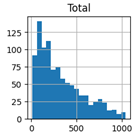
\includegraphics[width=\textwidth]{Chapters/ch1/n_dist_1.png}
        % \caption{Image A}
        % \label{fig:sub1}
    \end{subfigure}
    \hspace{0.05\textwidth} % Adjust the spacing between images
    \begin{subfigure}[b]{0.2\textwidth}
        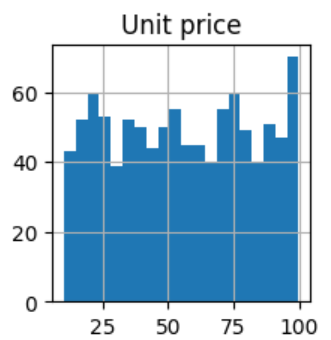
\includegraphics[width=\textwidth]{Chapters/ch1/unit-price.png}
        % \caption{Image B}
        % \label{fig:sub2}
    \end{subfigure}
    \hspace{0.05\textwidth} % Adjust the spacing between images
    \begin{subfigure}[b]{0.2\textwidth}
        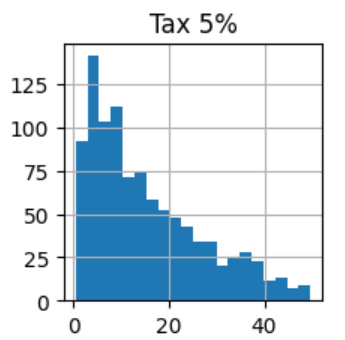
\includegraphics[width=\textwidth]{Chapters/ch1/tax.png}
        % \caption{Image C}
        % \label{fig:sub3}
    \end{subfigure}
    \hspace{0.05\textwidth} % Adjust the spacing between images
    \begin{subfigure}[b]{0.2\textwidth}
        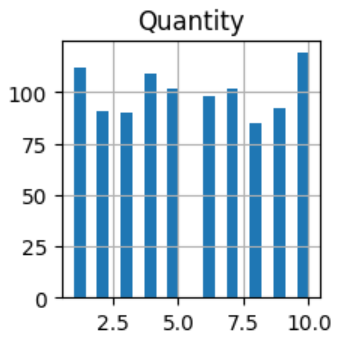
\includegraphics[width=\textwidth]{Chapters/ch1/quantity.png}
        % \caption{Image D}
        % \label{fig:sub4}
    \end{subfigure}
    % \caption{Four images in a row}
    % \label{fig:allimages}
\end{figure}




% If you are new to \LaTeX{}, there is a very good eBook -- freely available online as a PDF file -- called, ``The Not So Short Introduction to \LaTeX{}''. The book's title is typically shortened to just ``lshort''. You can download the latest version (as it is occasionally updated) from here:\\
% \href{http://www.ctan.org/tex-archive/info/lshort/english/lshort.pdf}{\texttt{http://www.ctan.org/tex-archive/info/lshort/english/lshort.pdf}}

% It is also available in several other languages. Find yours from the list on this page:\\
% \href{http://www.ctan.org/tex-archive/info/lshort/}{\texttt{http://www.ctan.org/tex-archive/info/lshort/}}

% It is recommended to take a little time out to learn how to use \LaTeX{} by creating several, small `test' documents. Making the effort now means you're not stuck learning the system when what you \emph{really} need to be doing is writing your thesis.

% \subsection{A Short Math Guide for \LaTeX{}}

% If you are writing a technical or mathematical thesis, then you may want to read the document by the AMS (American Mathematical Society) called, ``A Short Math Guide for \LaTeX{}''. It can be found online here:\\
% \href{http://www.ams.org/tex/amslatex.html}{\texttt{http://www.ams.org/tex/amslatex.html}}\\
% under the ``Additional Documentation'' section towards the bottom of the page.

% \subsection{Common \LaTeX{} Math Symbols}
% There are a multitude of mathematical symbols available for \LaTeX{} and it would take a great effort to learn the commands for them all. The most common ones you are likely to use are shown on this page:\\
% \href{http://www.sunilpatel.co.uk/latexsymbols.html}{\texttt{http://www.sunilpatel.co.uk/latexsymbols.html}}

% You can use this page as a reference or crib sheet, the symbols are rendered as large, high quality images so you can quickly find the \LaTeX{} command for the symbol you need.

% \subsection{\LaTeX{} on a Mac}
 
% The \LaTeX{} package is available for many systems including Windows, Linux and Mac OS X. The package for OS X is called MacTeX and it contains all the applications you need -- bundled together and pre-customised -- for a fully working \LaTeX{} environment and workflow.
 
% MacTeX includes a dedicated \LaTeX{} IDE (Integrated Development Environment) called ``TeXShop'' for writing your `\texttt{.tex}' files and ``BibDesk'': a program to manage your references and create your bibliography section just as easily as managing songs and creating playlists in iTunes.

%----------------------------------------------------------------------------------------
\newpage
{Initial correlation matrix for the dataset:}

\begin{figure}[h]
    \centering
    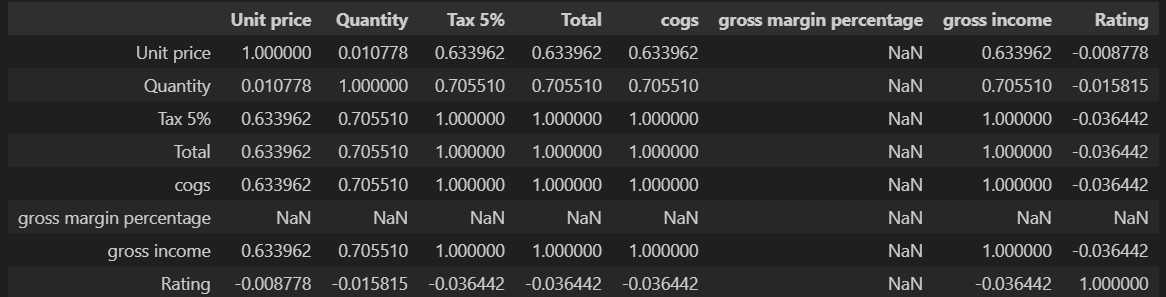
\includegraphics[width=1\textwidth]{Chapters/ch1/ch_1_corr_matrix.png}
    % \caption{This is an example image.}
    % \label{fig:example}
\end{figure}
% \subsection{About this Template}

We can observe a strong positive correlation between Unit Price, Quantity, Tax 5\%, Total, COGS, and Gross Income, suggesting that increases in one tend to correspond with increases in the others. However, the Gross Margin Percentage lacks variability in the given dataset, resulting in undefined correlations with other variables. Rating exhibits a very weak negative correlation with Unit Price, Quantity, Tax 5\%, Total, COGS, and Gross Income, implying that changes in Rating are not strongly associated with changes in these variables.


%----------------------------------------------------------------------------------------


\begin{figure}[h]
    \centering
    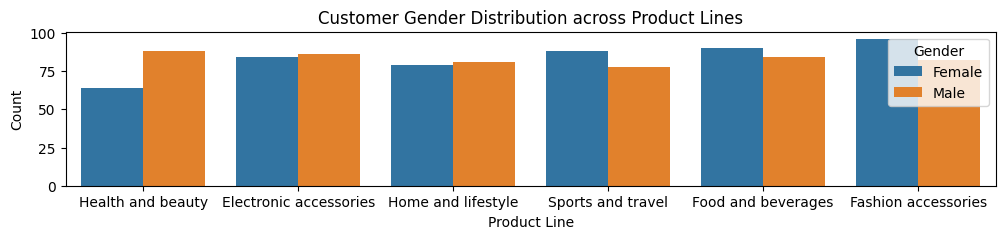
\includegraphics[width=1\textwidth]{Chapters/ch1/ch_1_barchart_1.png}
    % \caption{This is an example image.}
    % \label{fig:example}
\end{figure}
% \subsection{About this Template}

This helps understand how the purchase behavior varies between male and female customers for each product line. For example, it can reveal whether certain product lines are more popular among one gender, providing insights into potential marketing strategies or product positioning. If there's a significant gender bias in product preferences, the business can tailor its offerings accordingly.



%----------------------------------------------------------------------------------------


\begin{figure}[h]
    \centering
    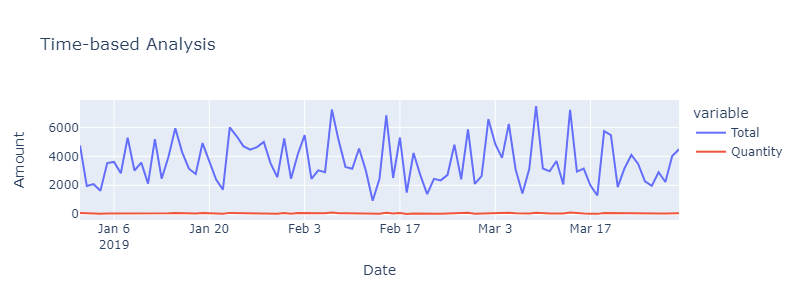
\includegraphics[width=1\textwidth]{Chapters/ch1/ch_1_timeseries_1.png}
    % \caption{This is an example image.}
    % \label{fig:example}
\end{figure}
% \subsection{About this Template}
The line plot shows the overall trend of total sales and quantity sold over the given time.The sharp dips and spikes indicate the variance of the ‘Total’ feature. And the almost-straight, red line indicates, with its stagnancy, a low variation in the feature ‘Quantity’ throughout the months January to March.


%----------------------------------------------------------------------------------------


\begin{figure}[h]
    \centering
    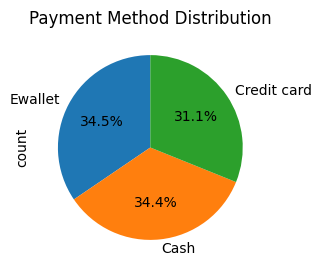
\includegraphics[width=0.5\textwidth]{Chapters/ch1/ch_1_pie_chart_1.png}
    % \caption{This is an example image.}
    % \label{fig:example}
\end{figure}
% \subsection{About this Template}
 This Pie Chart visualization provides insights into the preferred payment methods of customers. Understanding the dominant payment method is crucial for optimizing payment processing systems and ensuring that the most convenient options are available. It also indicates trends in customer preferences and potentially influences decisions related to partnerships with specific payment providers. As can be seen by this chart, all 3 payment modes are near-to-identical and hence preferred almost equally by customers.

%----------------------------------------------------------------------------------------

\begin{figure}[h]
    \centering
    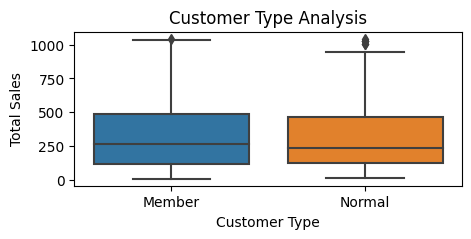
\includegraphics[width=0.8\textwidth]{Chapters/ch1/ch_1_box_plot_1.png}
    % \caption{This is an example image.}
    % \label{fig:example}
\end{figure}
% \subsection{About this Template}

This provides a visual summary of the distribution of total sales for each customer type. There seem to be few outliers beyond the whiskers, indicating high sales for a few examples. Outliers for non-members could indicate specific cases where non-members made exceptionally high purchases.


%----------------------------------------------------------------------------------------

{Exploring the performance of each branch based on total sales and average ratings:}

\begin{figure}[h]
    \centering
    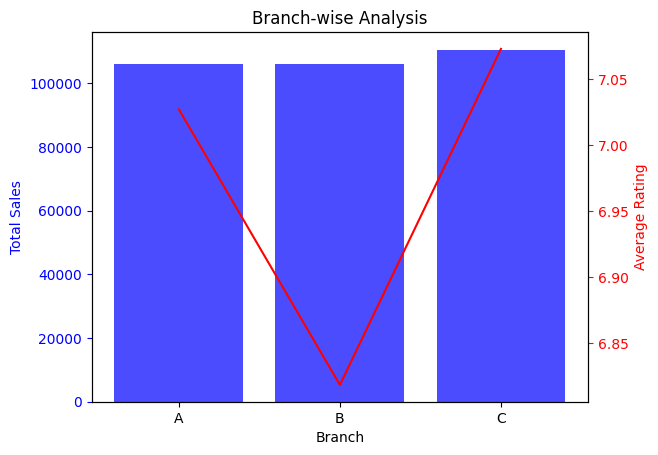
\includegraphics[width=0.5\textwidth]{Chapters/ch1/ch_1_barchart_2.png}
    % \caption{This is an example image.}
    % \label{fig:example}
\end{figure}
% \subsection{About this Template}

The blue bars represent the total sales for each branch. The branches here seem to be almost identical in terms of Sales, with Branch C leading the other by just a bit.
The red line represents the average rating for each branch. This helps evaluate the average customer satisfaction (rating) for each branch. An interesting thing to note is the steep descent of Average Rating for Branch B. This indicates that Branch A has the highest average rating, followed by Branch C. Relatively, Branch B has quite a low average rating.
Grouping by Branch:
\begin{lstlisting}[language=Python, frame=none]
branch_analysis = df.groupby('Branch').agg({'Total': 'sum', 'Rating': 'mean'}).reset_index()
\end{lstlisting}
The code groups the dataset by the 'Branch' column, calculating the total sales and average rating for each branch.

%----------------------------------------------------------------------------------------



\begin{figure}[h]
    \centering
    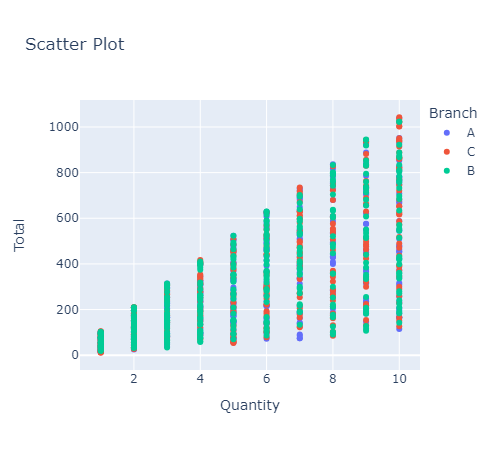
\includegraphics[width=0.5\textwidth]{Chapters/ch1/ch_1_scatter_plot_1.png}
    % \caption{This is an example image.}
    % \label{fig:example}
\end{figure}
% \subsection{About this Template}
This scatter plot represents the relationship between the 'Quantity' and 'Total' columns, with each point corresponding to a specific invoice. The color of the points is differentiated based on the 'Branch' column, and additional information about the 'Product line' is available when hovering over each point in the ipynb file.
This interactive plot allows us to explore the relationship between the quantity and total sales.



% Chapter 1

\chapter{Data Preprocessing} % Main chapter title

\label{Chapter2} % For referencing the chapter elsewhere, use \ref{Chapter1} 

\lhead{\emph{Data Preprocessing}} % This is for the header on each page - perhaps a shortened title

%----------------------------------------------------------------------------------------

\section{Data Cleaning}

 I made use of relevant function in Pandas to check for missing values, duplicates, and outliers. However, the data was quite clean already, and barely required any initial cleaning. The table below shows no null values in any of the columns:

\begin{table}[htbp]
    \centering
    \rowcolors{1}{orange!20}{white}
    \begin{tabular}{|>{\columncolor{orange!50}}c|c|}
        \hline
        \rowcolor{orange!50}
        \textbf{Column Name} & \textbf{Total Null Values} \\
        \hline
        Invoice ID & 0 \\
        Branch & 0 \\
        City & 0 \\
        Customer type & 0 \\
        Gender & 0 \\
        Product line & 0 \\
        Unit price & 0 \\
        Quantity & 0 \\
        Tax 5\% & 0 \\
        Total & 0 \\
        Date & 0 \\
        Time & 0 \\
        Payment & 0 \\
        COGS & 0 \\
        Gross margin percentage & 0 \\
        Gross Income & 0 \\
        Rating & 0 \\
        \hline
    \end{tabular}
    \caption{There were no duplicates or outliers}
    \label{tab:alternating_colors}
\end{table}

% If you are writing a thesis (or will be in the future) and its subject is technical or mathematical (though it doesn't have to be), then creating it in \LaTeX{} is highly recommended as a way to make sure you can just get down to the essential writing without having to worry over formatting or wasting time arguing with your word processor.

% \LaTeX{} is easily able to professionally typeset documents that run to hundreds or thousands of pages long. With simple mark-up commands, it automatically sets out the table of contents, margins, page headers and footers and keeps the formatting consistent and beautiful. One of its main strengths is the way it can easily typeset mathematics, even \emph{heavy} mathematics. Even if those equations are the most horribly twisted and most difficult mathematical problems that can only be solved on a super-computer, you can at least count on \LaTeX{} to make them look stunning.

%----------------------------------------------------------------------------------------

\section{DateTime}

The main task here was to make use of the existing Date and Time features and extract utilizable features. Other than this, I dropped a few irrelevant columns in the preprocessing phase. After doing so, I was able to get the following new features:


\begin{table}[htbp]
    \begin{minipage}{0.45\linewidth}
        \centering
        \rowcolors{1}{green!20}{white}
        \begin{tabular}{|>{\columncolor{green!50}}c|c|}
            \hline
            \rowcolor{green!50}
            \textbf{Date} & \cellcolor{green!50}\textbf{Time} \\
            \hline
            1/5/2019 & 13:08 \\
            3/8/2019 & 10:29 \\
            3/3/2019 & 13:23 \\
            1/27/2019 & 20:33 \\
            2/8/2019 & 10:37 \\
            \hline
        \end{tabular}
        \caption{Original Features}
        \label{tab:alternating_colors}
    \end{minipage}
    \hfill
    \begin{minipage}{0.45\linewidth}
        \centering
        \rowcolors{1}{green!20}{white}
        \begin{tabular}{|>{\columncolor{green!50}}c|c|c|}
            \hline
            \rowcolor{green!50}
            \textbf{Date} & \cellcolor{green!50}\textbf{Time} & \cellcolor{green!50}\textbf{Duration} \\
            \hline
            1 & 3 & 13 \\
            3 & 8 & 10 \\
            3 & 3 & 13 \\
            1 & 27 & 20\\
            2 & 8 & 10 \\
            \hline
        \end{tabular}
        \caption{New Features}
        \label{tab:extended_features}
    \end{minipage}
\end{table}



%----------------------------------------------------------------------------------------

\section{Encoding}

The main task here was to make use of the existing Date and Time features and extract utilizable features. Other than this, I dropped a few irrelevant columns in the preprocessing phase. After doing so, I was able to get the following new features:

\vspace{2cm}

\begin{table}[htbp]
    \centering
    \rowcolors{1}{orange!20}{white}
    \begin{tabular}{|>{\columncolor{orange!50}}c|c|}
        \hline
        \rowcolor{orange!50}
        \textbf{Column Name} & \textbf{Total Null Values} \\
        \hline
        Branch & 3 \\
        City & 3 \\
        Customer type & 2 \\
        Gender & 2 \\
        Product line & 6 \\
        Unit price & 943 \\
        Quantity & 10 \\
        Tax 5\% & 990 \\
        Total & 990 \\
        Payment & 3 \\
        COGS & 990 \\
        Gross margin percentage & 1 \\
        Gross Income & 990 \\
        Rating & 61 \\
        \hline
    \end{tabular}
    % \caption{there were no duplicates or outliers}
    \label{tab:alternating_colors}
\end{table}



\begin{figure}[h]
    \centering
    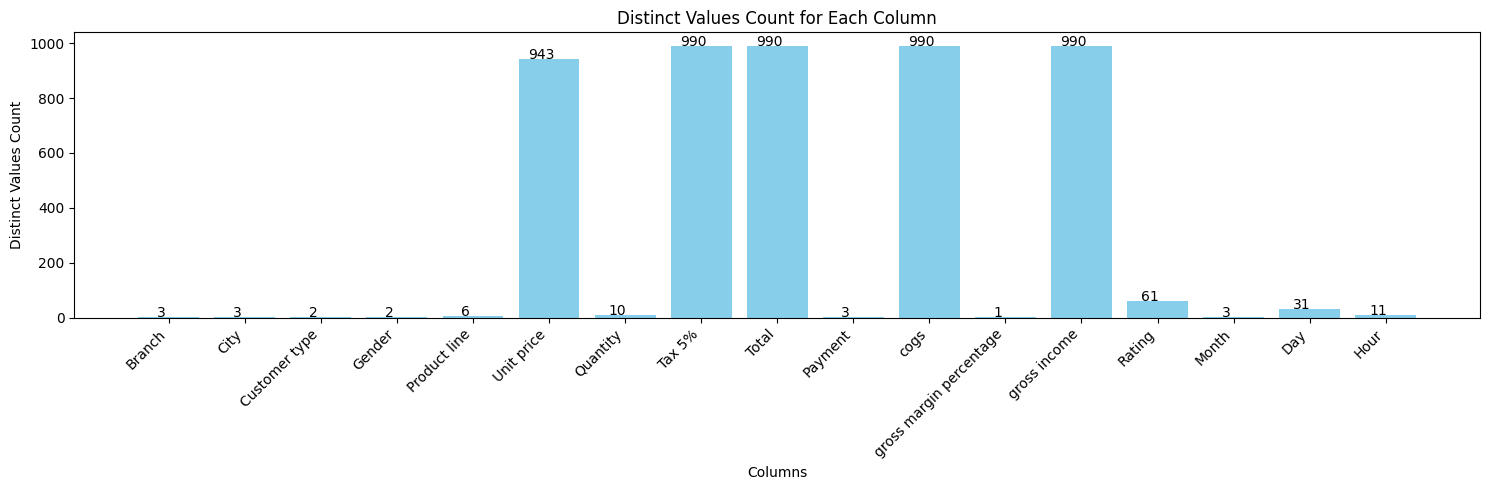
\includegraphics[width=1\textwidth]{Chapters/ch2/testing .png}
    % \caption{This is an example image.}
    % \label{fig:example}
\end{figure}
% \subsection{About this Template}

\newpage 
From this we can identify the feature ‘gross margin percentage’ is not of any use, since it has only 1 distinct value. Which means it cannot have any correlation with other features, hence, it will not hold any importance in the variation of any target variable that we may choose when training a model.

\begin{table}[htbp]
    \centering
    \resizebox{\textwidth}{!} & \textbf{Total} & \textbf{Unit price} & \textbf{COGS} & \textbf{Gross income} \\
        \hline
        \textbf{Total} & 0.002515 & 0.00277 & 0.022301 & 0.70551 & 0.036442 & 1.0 & 1.0 & 0.633962 & 1.0 & 1.0 \\
        \hline
        
    \end{tabular}%
    }
    % \caption{Scaled Table with Headers, Larger Font, and Wider Rows}
    \label{tab:scaled_table}
\end{table}



\subsection{Label Encoding}

suitable for ordinal variables, where there is an inherent order or ranking among the categories. For example, in our dataset, the days are ordinal because they have a clear and meaningful sequence. Each day follows the previous one in a systematic and sequential manner. Label encoding assigns integers based on this order, with the assumption that there is a linear relationship between the categories. This simplifies the representation of this variable while preserving the ordinal information. Hence, I’m using Label Encoding for the columns ‘Day’, ‘Month’ and ‘Hour.

\subsection{One Hot Encoding}

suitable for nominal variables, where there is no inherent order among the categories. Nominal variables represent categories with no implied order or ranking. In our dataset, columns like 'Branch', 'City', 'Gender', 'Product line', ‘Customer type’, and 'Payment' fall into this category.
\newline

The decision to use one-hot encoding is influenced by the understanding that these variables represent categories without any natural order. One-hot encoding creates binary columns for each category, providing a binary indicator (0 or 1) for the presence of each category. This is crucial to avoid introducing false ordinal relationships in the data.

%----------------------------------------------------------------------------------------

\section{Standardization}

\subsection{Why was Standardization required here?}

It is necessary to ensure that all features contribute equally to the analysis or model training, as many machine learning algorithms are sensitive to the scale of the input features. Standardization transforms the data so that it has a mean of 0 and a standard deviation of 1, making it easier for algorithms to converge and improving the interpretability of coefficients.

% to set the margin of the subsection 

% comment out this
% \titleformat{\subsubsection}[hang]{\normalfont\bfseries}{\hspace{2em}\thesubsubsection}{1em}{}

\subsubsection{Visual Insepection}

\textbf{a) Histogram:} 
\begin{figure}[h]
    \centering
    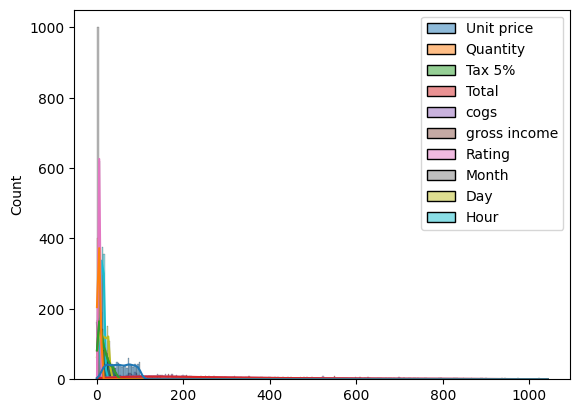
\includegraphics[width=0.5\textwidth]{Chapters/ch2/ch_2_line_graph_1.png}
    % \caption{This is an example image.}
    % \label{fig:example}
\end{figure}

Clearly, the histogram is not totally symmetric. Histograms depicting normal distribution show bell-shaped curves, and this is not bell-shaped. Hence, the data is not normally distributed.

\textbf{b) Quantile-Quantile (Q-Q) Plot} 
\newline 
\begin{figure}[h]
    \centering
    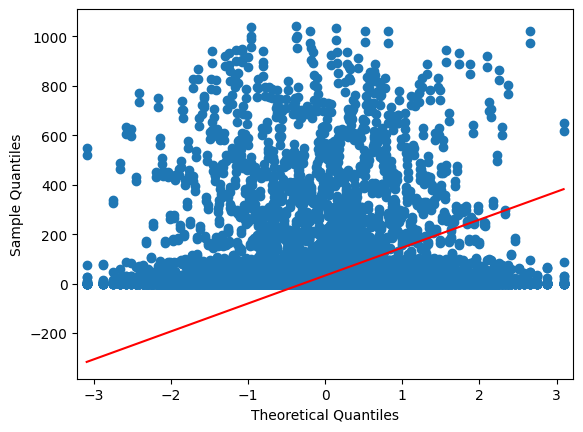
\includegraphics[width=0.5\textwidth]{Chapters/ch2/ch_2_scatter_plot_1.png}
    % \caption{This is an example image.}
    % \label{fig:example}
\end{figure}

In a Q-Q plot, if the points fall approximately along a straight line, the data is likely normally distributed. As can be seen clearly here, this is not the case. Deviations from the straight red line suggest departures from normality. 
\newline
Hence, by both the visual inspections we have inferred that the dataset is not normally distributed. 
Another way of checking for data normality is by conducting statistical tests. 

\subsubsection{Statistical Test (Shapiro-Wilk Test) }
Upon conducting this test on our dataset, I got the following output: 
\newline
Shapiro-Wilk Test: Statistic = 0.31571829319000244, p-value = 0.0
\newline
Since the p-value is lower than the chosen significance level (0.05), we can reject the null hypothesis; the data is not normally distributed.
\newline
Hence, both the visual and statistical tests have led us to believe that the data is not normally distributed and hence required normalization or standardization. But which one is suitable for our specific dataset and why?

\subsection{Which Features require Standardization and why?}
Standardization becomes essential when examining features with numeric values, especially those displaying significant scale variations. The features that benefited from standardization include:


\begin{itemize}
\item Unit price: The prices of different products can vary widely, and standardizing this feature ensures that the magnitude of the price doesn't disproportionately influence other features during model training.
\item Quantity: The number of items purchased can also exhibit considerable variability, and standardization aids in rendering this feature comparable with others.
\item Tax 5\%, Total, cogs, gross income: These features represent monetary values and may have different scales. Standardization is instrumental in ensuring that these monetary metrics are on a consistent scale, facilitating fair comparison.
\item Rating: While this feature might not necessarily demand standardization if it already falls within a specific range, if the rating scale significantly differs from other features, standardization becomes beneficial in maintaining uniformity across all features.
\end{itemize}

\subsection{Choosing between Normalization and Standardization}
\begin{itemize}
\item Magnitude Differences: Standardization is robust to features with different scales, making it suitable for datasets where features like "Unit price," "Quantity," etc., may have different magnitudes.
\item Outliers: Standardization is less sensitive to outliers compared to normalization, which can be beneficial in real-world datasets that might have some outliers.
\item Algorithms Sensitivity: Many machine learning algorithms, including those used in data mining, can benefit from standardized features, especially when they involve calculations of distances or gradients.
\end{itemize}


\subsection{Using StandardScaler}
Before applying standardization, it is important to exclude the target column. Since we want to predict target values as they are in the original dataset, we do not apply any preprocessing like encoding or standardization to the target variable. The code involved in the actual standardization is basically 2 lines:
\begin{lstlisting}[language=Python, frame=none]
scaler = StandardScaler()
df_standardized[features] = scaler.fit_transform(df_standardized[features])
\end{lstlisting}

This code creates an instance of the StandardScaler class from scikit-learn. The StandardScaler is a transformer that standardizes features by removing the mean and scaling to unit variance. 
The \verb|fit_transform| method calculates the mean and standard deviation of each selected column and then applies the standardization formula:
\begin{equation}
Standardized Value = Original Value-Mean/Standard Deviation
\end{equation}

\begin{figure}[h]
    \centering
    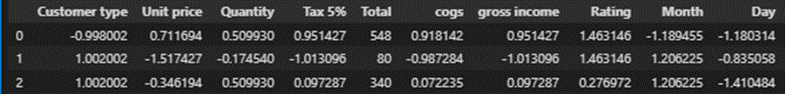
\includegraphics[width=1\textwidth]{Chapters/ch2/data_1.png}
    \caption{Sample of a few features from the standardized dataset}
    % \label{fig:example}
\end{figure}

\subsection{How did this step contribute to effective data mining?}

\begin{itemize}
\item Improved Model Convergence: Standardizing features helped machine learning models converge faster during training, especially for algorithms that relied on gradient descent optimization.
\item Enhanced Model Performance: Standardization ensured that each feature contributed equally to the model, preventing features with larger scales from dominating the learning process. This led to better model performance and generalization.
\item Facilitated Interpretation: Standardization made it easier to interpret the coefficients of the features in linear models. This was important for understanding the impact of each feature on the target variable.
\item Increased Robustness: Scaling using StandardScaler made models more robust to variations in the data and helped avoid numerical instability issues during training data and helped avoid numerical instability issues during training.
\end{itemize}

% ---------------------------------------------------------------------------------------------------

\section{Feature Selection } 
I employed PCA to conduct feature selection. Technically, PCA makes use of both feature selection and creation. It basically ‘merges’ the top ‘k’ features together, where ‘k’ is user-defined. 
The motivation for using PCA specifically was simply because we had been taught that in depth, and I wanted to try it out. Choosing ‘k’ was the main factor.



\subsection{Choosing K}
As I mentioned above, ‘k’ is the number of principal components that we are choosing to work with. Choosing this value can be a challenging task, and I utilized various means to try and understand what the ideal value could be.

\begin{figure}[h]
    \centering
    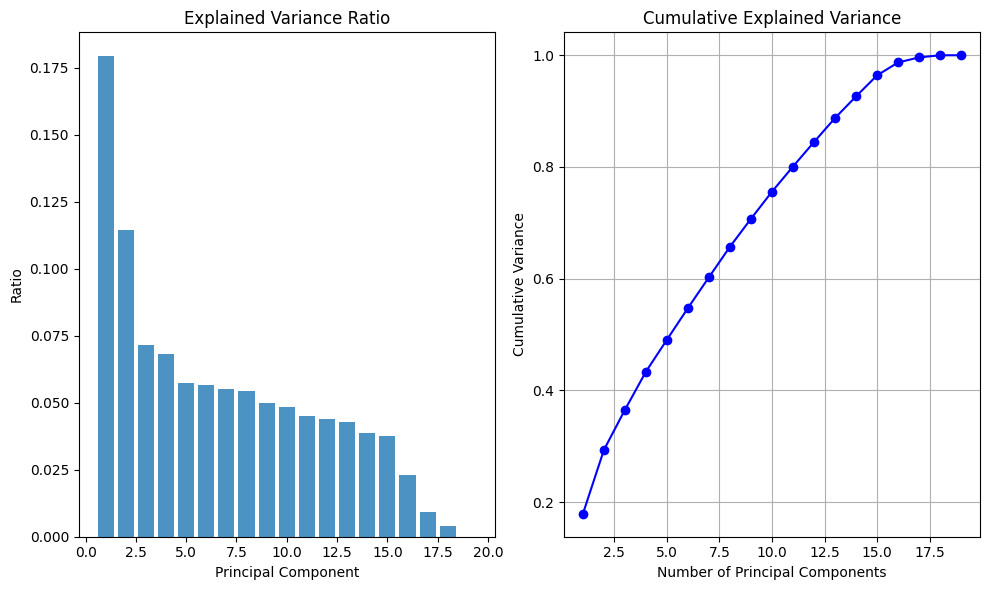
\includegraphics[width=0.7\textwidth]{Chapters/ch2/ch2_vr_er_1.png}
    % \caption{This is an example image.}
    % \label{fig:example}
\end{figure}
\begin{figure}[h]
    \centering
    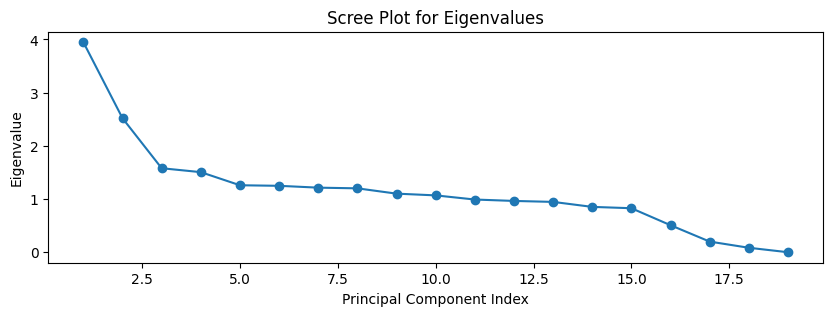
\includegraphics[width=0.7\textwidth]{Chapters/ch2/ch_2_screeplot_1.png}
    % \caption{This is an example image.}
    % \label{fig:example}
\end{figure}
\newpage
After analyzing these charts, I decided to initially start by experimenting with ‘k’ at 15. The most efficient way of finding the ideal value for ‘k’ is by trial and error. But using these means can help figure out a good starting point.
% -----------------------------------------------------------------------------------------------------


\section{Splitting Data}

\subsection{Importance of splitting}

\begin{itemize}
\item Avoids Overfitting: Imagine training your model on the same data you use to evaluate it. It would be like memorizing the answers in a test instead of truly understanding the concepts. The model might perform well on that specific data (high training accuracy), but it wouldn't generalize well to new, unseen data (low testing accuracy). Splitting the data prevents this "memorization" by reserving the testing set for unbiased evaluation.
\item Provides Unbiased Evaluation: Training the model only on the training set eliminates any influence from the testing data. This ensures the evaluation metrics (e.g., R-squared, mean squared error) reflect the model's true performance on unseen data, making it a reliable measure of its generalizability.
\item Helps Tune Hyperparameters: Hyperparameters are knobs that influence the model's learning process. Splitting the data allows you to experiment with different hyperparameter values on the training set, evaluating their impact on performance through the validation set, and finally selecting the best performing configuration for the final model.
\item Identifies Data Leakage: Data leakage occurs when information from the testing set somehow influences the training process. For example, including future values in a time series prediction might give the model an unfair advantage in training. Splitting the data minimizes this risk and leads to a more accurate assessment of the model's true capabilities.
\item Facilitates Cross-Validation: Splitting the data can be extended to cross-validation techniques, where the dataset is further divided into multiple folds. Each fold is used for training and testing in turn, providing a more robust and statistically sound evaluation of the model's performance across different data subsets.
\end{itemize}
% =================================================
\subsection{Applying Train-Test Split}

The \verb|train_test_split| function from the \verb|scikit-learn| library is used to split the data into training and testing sets. The parameters are as follows:
\begin{itemize}

\item X: The feature matrix (The preprocessed DataFrame)
\item y: The target variable (‘Total’)
\item \verb|test_size|: The proportion of the dataset to include in the test split. In this case, it's set to 0.2, meaning 20\% of the data will be used for testing.
\item \verb|random_state|: This is used to ensure reproducibility. Setting a seed (here, 42) means that if you run the code multiple times, you'll get the same train-test split each time.

\end{itemize}

The resulting dimensions of both sets:
\verb|X_train shape: (800, 22)|,
\verb|X_test shape: (200, 22)|,
\verb|y_train shape: (800,)|,
\verb|y_test shape: (200,)|


% --------------------------------------------------------------------------------------------------------


% Chapter 1

\chapter{Visualization} % Main chapter title

\label{Chapter3} % For referencing the chapter elsewhere, use \ref{Chapter1} 

\lhead{Chapter 3. \emph{Visualization}} % This is for the header on each page - perhaps a shortened title

%----------------------------------------------------------------------------------------

\section{Variable Distributions and Patterns }

\subsection{Numerical Variable Distributions:}
For numerical variables like 'Unit price,' 'Quantity,' 'Tax 5\%,' 'Total,' etc., their distributions can be visualized using histograms. Histograms show how the values are spread across different ranges or bins. Important aspects to consider include:
Central Tendency: Is the distribution centered around a particular value (mean or median)?
Spread: How spread out are the values? Are there outliers?
Shape: Does the distribution have a particular shape, such as normal, skewed, or bimodal?

\subsection{Categorical Variable Distributions}
For categorical variables like 'Branch,' 'City,' 'Customer type,' 'Payment,' etc., their distributions can be visualized using count plots or bar charts. These plots show the frequency of each category. Important considerations include:
{\begin{itemize}
    \item Frequency: Which categories are most common or rare?
    \item Imbalances: Are there significant imbalances in the distribution of categories?
\end{itemize}}
Frequency: Which categories are most common or rare?
    \item Imbalances: Are there significant imbalances in the distribution of categories?

\subsection{Bivariate Relationships}
Exploring relationships between variables, especially between numerical and categorical variables, helps understand how variables interact. Box plots, pair plots, or other bivariate visualizations provide insights into how the distribution of a numerical variable varies across different categories of a categorical variable.

\subsection{Time Trends}
For temporal variables like 'Date' in a time series dataset, understanding the distribution involves looking at how values change over time. Time series plots can reveal trends, seasonality, or patterns in the data.


% ---------------------------------------------------------------------------------------------------------

\section{Why is Visualization required here?} 
Visualizations are a cornerstone of data exploration and communication. They play a crucial role in this project by doing the following.

\subsection{Unveiling Hidden Patterns and Relationships}
\begin{itemize}
\item Revealing trends, correlations, and anomalies that might be obscured in raw data tables.
\item Exposing patterns in customer behavior, product preferences, sales patterns, and seasonal influences.
\item Highlighting relationships between variables, such as the impact of promotions on sales or the influence of customer demographics on purchasing habits.
\end{itemize}


\subsection{Enhancing Understanding and Communication}
\begin{itemize}

\item Transforming complex data into intuitive and accessible visual representations. 
\item Making insights easier to comprehend, interpret, and share among stakeholders with varying levels of technical expertise.
\item Fostering collaboration and discussion by providing a visual platform for exploration and debate.
\end{itemize}

\subsection{Guiding Further Analysis and Decision-Making:}
\begin{itemize}

\item Informing subsequent steps in the data mining process, such as feature selection, model building, and evaluation.
\item Supporting data-driven decision-making by providing evidence-based insights for marketing strategies, inventory management, customer segmentation, and other business initiatives.	

\end{itemize}
% --------------------------------------------------------------------------------------------------

\section{Visualizations }

\begin{figure}[h]
    \centering
    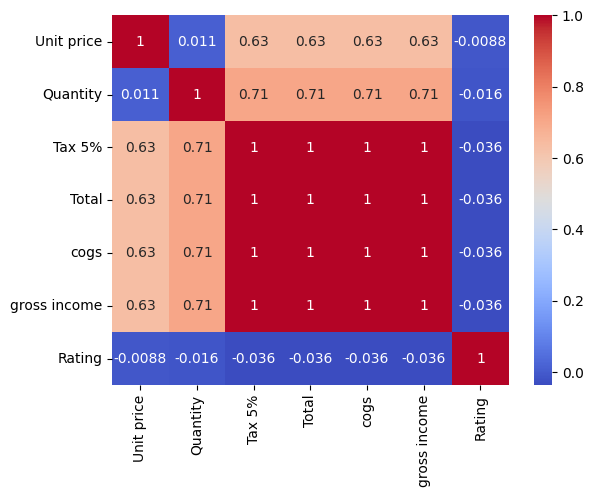
\includegraphics[width=0.7\textwidth]{Chapters/ch3/ch_3_heatmap.png}
    \caption{Correlation Matrix Heatmap}
    % \label{fig:example}
\end{figure}

Features like Tax, Total, Cost of Goods Sold, and Gross Income, can be seen having maximum positive correlation- which means they are highly directly correlated. Most other features are also highly correlated in a positive manner. Rating is slightly negatively correlated with all other features.

\begin{figure}[h]
    \centering
    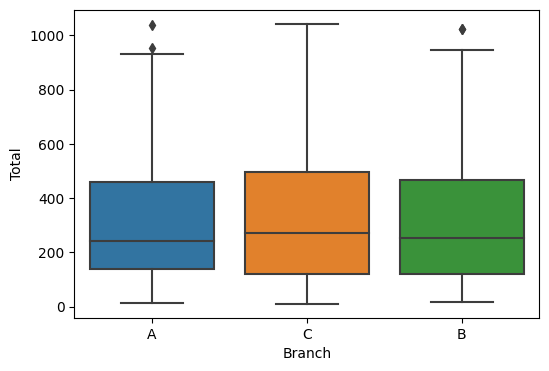
\includegraphics[width=0.7\textwidth]{Chapters/ch3/ch_3_boxplot.png}
    \caption{Box plot by branch}
    % \label{fig:example}
\end{figure}
The distribution of the ‘Total’ column by Branch can be observed here. All Branches seem to have a higher distribution of values for ‘Total’ from the 50th to 75th percentile (middle to Q3). This means that all branches have higher totals per average transaction. How high though? As can be seen from the boxplots, the trend of higher distribution of values starts from around the \$200 mark. 

\begin{figure}[h]
    \centering
    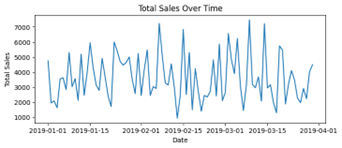
\includegraphics[width=0.7\textwidth]{Chapters/ch3/tim_s_1.png}
    \caption{Time series graph}
    % \label{fig:example}
\end{figure}
The plot reveals the overall trend of total sales across all three branches over time. It allows us to identify seasonal patterns in sales, such as fluctuations due to holidays or periods of high demand. It reveals higher trends in sales patterns, such as in mid-February and mid-March, that could indicate significant events or changes in store operations.

\begin{figure}[h]
    \centering
    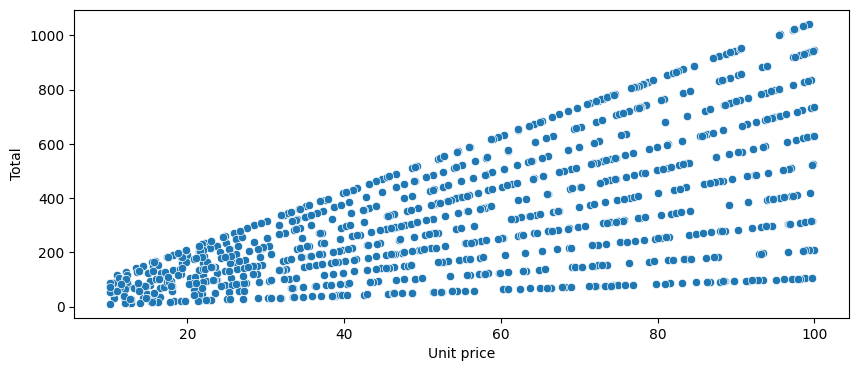
\includegraphics[width=0.7\textwidth]{Chapters/ch3/ch_3_scatterplot.png}
    \caption{Scatter plot}
    % \label{fig:example}
\end{figure}
Each point represents a single transaction, positioned according to its unit price and total value. Here we can observe a clear positive correlation, as values for ‘Total’ tend to increase with ‘Unit Price’. Not only this, but the density of points (transactions) also sees an upward trend as both features increase in their respective magnitudes.

\begin{figure}[h]
    \centering
    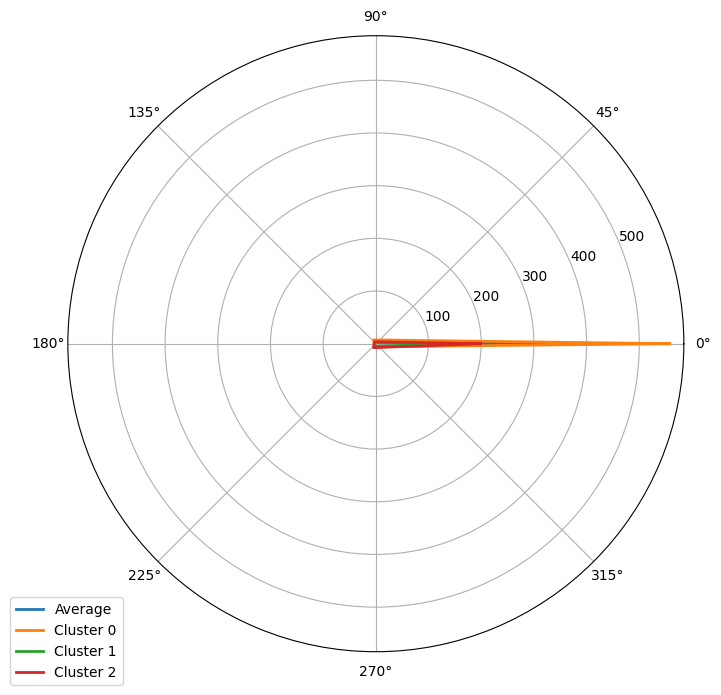
\includegraphics[width=0.7\textwidth]{Chapters/ch3/ch_3_spiral.png}
    \caption{Radar graph}
    % \label{fig:example}
\end{figure}
\newpage
To make this, I selected specific features ('Total', 'Quantity', 'Rating') for segmentation. After this I standardized the features and then using K-Means, performed clustering (3 clusters). Each cluster represents a group of transactions with similar characteristics in terms of these variables. This helps identify distinct segments or groups within the data, allowing for a more nuanced understanding of how certain features contribute to the segmentation. Cluster 0 (represented by the outermost line in orange) covers most of the radar chart, occupying about 2/5ths of the outermost line. This suggests that a significant portion of the 3 features fall into Cluster 0. Cluster 1 is visible as a green segment for about 1/5th of the outer line. This indicates that there is a distinct group of data points (transactions) in Cluster 1 with specific characteristics that differentiate them from other clusters. Similarly, Cluster 2 is represented by a red segment for about 1/5th of the outer line. This suggests another distinctive group of data points with different characteristics compared to the rest of the dataset. The dominance of Cluster 0 suggests that it has a larger influence on the overall dataset. The cyclical appearance of different colored segments may indicate temporal patterns in customer behavior.

\begin{figure}[h]
    \centering
    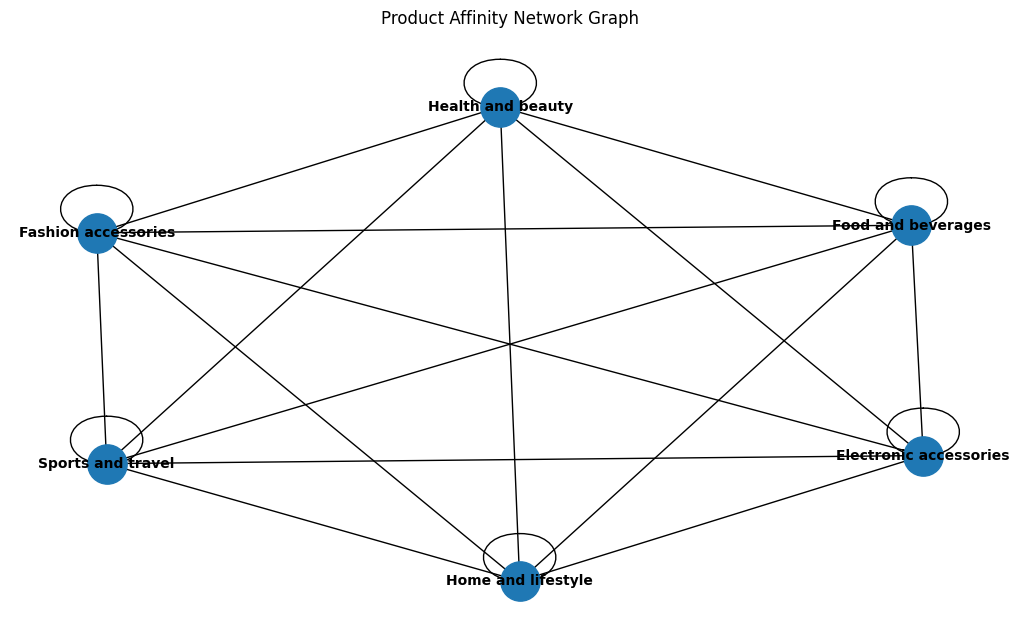
\includegraphics[width=0.7\textwidth]{Chapters/ch3/ch_3_graph.png}
    \caption{Product affinity network graph}
    % \label{fig:example}
\end{figure}
\newpage
An undirected graph G is created using nx.Graph(). This graph represents relationships between products. The pairs of products represent the sequence of products in the 'Product line' column. Edges are added to the graph (G) using \verb|G.add_edges_from(pairs)|. Each pair of consecutive products in the 'Product line' forms an edge in the graph. The graph helps identify which products are often purchased together or follow each other in sales transactions. Each node here is connected to every other node which suggests a high level of interconnectedness. In the context of product affinity, it implies a strong association between all pairs of product lines. Hence, there are no specific clusters or groups of product lines; rather, all product lines are somewhat related to each other.




% Chapter 4

\chapter{Association Rule Mining} % Main chapter title

\label{Chapter4} % For referencing the chapter elsewhere, use \ref{Chapter1} 

\lhead{Chapter 4. \emph{Association Rule Mining}} % This is for the header on each page - perhaps a shortened title
Apriori cannot be applied directly to the dataset. There are certain processes a dataset must go through before we can apply the algorithm. I chose to manually prepare the data to better understand and document the entire process.
%----------------------------------------------------------------------------------------

\section{Data preparation }

\subsection{Creating a list of lists}
First, I selected the ‘Product line’ feature from the dataset, as this was going to be the focus when implementing Apriori on the dataset. I split each element in the 'Product line' column into a list of substrings using the string ' and ' as the separator. After this, I used the Pandas function ‘.explode’ to transform each element of a list-like to a row, replicating the index values. Finally, I converted the Pandas Series to a list. All these steps were performed in this single line of code:
\begin{lstlisting}[language=Python, frame=none]
exploded_list = apriori_df['Product line'].str.split(' and ').explode().tolist()
\end{lstlisting}

\subsection{Grouping products by count}
I used the list of lists to create a Pandas DataFrame, and then added a new column ‘Count’ to this DataFrame. Using ‘groupby’ and ‘transform’, I was able to count the frequency of each product. Finally, I removed any duplicates to retain only the unique products ad their corresponding counts.

\subsection{Encoding the DataFrame using Transaction Encoder}
The transaction encoder is also part of the mlxtend library and can be imported and directly used in Python to encode features based on their frequencies. Using the ‘fit’ method in ‘tx.fit’ along with ‘transform’, I was able to transform the data into a binary encoded array. 2 main changes made after this are to convert the array into a DataFrame, and to convert the binary values to an integer form (0s and 1s). Now, the dataset is finally ready as input to the Apriori algorithm.

\section{Frequent Itemsets}

\subsection{Calculation}

‘Apriori’ is a function from the \verb|mlxtend.frequent_patterns|’ module, specifically designed for implementing the Apriori algorithm. I made use of it at this stage to apply the apriori algorithm to our dataset, with the objective of forming frequent itemsets. What exactly are frequent itemsets? Put simple, they are sets of items that appear together frequently in a dataset. Another term I’ll use here is minimum support, which measures the proportion of transactions in which an itemset occurs in a dataset. I set the ‘\verb|min_support|’ parameter to 0.01 (1\%), which specifies the minimum support threshold. Here, the ‘\verb|min_support|’ parameter filters out infrequent itemsets, considering only those that occur with a frequency greater than or equal to 0.01.
% ============================
\subsection{Choosing Minimum Support}
To answer this question, we must consider the ‘products by their counts’ DataFrame that I formed while preparing the data:

\begin{table}[htbp]
    \centering
    \rowcolors{1}{blue!20}{white}
    \begin{tabular}{|>{\columncolor{blue!50}}c|c|}
        \hline
        \rowcolor{blue!50}
        \textbf{Product} & \textbf{Count} \\
        \hline
        Health & 152 \\
        Beauty & 152 \\
        Electronic accessories & 170 \\
        Home & 160 \\
        Lifestyle & 160 \\
        Sports & 166 \\
        Travel & 166 \\
        Food & 174 \\
        Beverages & 174 \\
        Fashion Accessories & 178 \\
        \hline
    \end{tabular}
    % \caption{there were no duplicates or outliers}
    \label{tab:alternating_colors}
\end{table}

The counts for each product line indicate that the dataset covers a variety of product lines, and there's a reasonable distribution of counts across different categories. Setting a minsup of 0.01 means that we are considering itemsets that appear in at least 1\% of the transactions. Since the entire dataset consists of a total of 1000 rows, this translates to a minimum count of 10 transactions. Considering that the lowest count is 152, a minsup of 0.01 seems reasonable as it is significantly above the minimum count of any individual product line, implying that we are capturing product lines which are relatively common in the dataset.
\newline
The choice of 0.01 strikes a balance between generality and specificity. It's low enough to capture patterns that occur frequently but high enough to avoid capturing extremely specific patterns. A lower minsup also allows for the discovery of a larger number of frequent itemsets, providing a more general view of patterns in the data.
% ===================================================================================


\subsection{The frequent itemset produced}
The resultant DataFrame (\verb|frequent_itemsets|) contains frequent itemsets along with their support values.

\begin{table}[htbp]
    \centering
    \rowcolors{1}{blue!20}{white}
    \begin{tabular}{|>{\columncolor{blue!50}}c|c|}
        \hline
        \rowcolor{blue!50}
        \textbf{Support} & \textbf{Itemsets} \\
        \hline
        0.166667 & (Electronic accessories) \\
        0.166667 & (Fashion accessories) \\
        0.166667 & (Food) \\
        0.166667 & (Health) \\
        0.166667 & (Home) \\
        0.166667 & (Sports) \\
        0.166667 & (Beauty) \\
        0.166667 & (Beverages) \\
        0.166667 & (Lifestyle) \\
        0.166667 & (Beverages, Food) \\
        0.166667 & (Health, Beauty) \\
        0.166667 & (Lifestyle, Home) \\
        0.166667 & (Travel, Sports) \\
        \hline
    \end{tabular}
    % \caption{there were no duplicates or outliers}
    \label{tab:alternating_colors}
\end{table}


The itemsets of individual products (Electronic accessories), (Fashion accessories), (Food), (Health), (Home), (Sports), (beauty), (beverages), (lifestyle), and (travel) all have a support of 0.166667 (16.67\%). This means that each of these product lines individually appears in approximately 16.67\% of the transactions.
\newline
As for 2-itemsets: (beverages, Food), (Health, beauty), (lifestyle, Home), and (travel, Sports); each have a support of 0.166667 (16.67\%), indicating that these pairs of product lines occur together in approximately 16.67\% of the transactions.


% If you are writing a thesis (or will be in the future) and its subject is technical or mathematical (though it doesn't have to be), then creating it in \LaTeX{} is highly recommended as a way to make sure you can just get down to the essential writing without having to worry over formatting or wasting time arguing with your word processor.

% \LaTeX{} is easily able to professionally typeset documents that run to hundreds or thousands of pages long. With simple mark-up commands, it automatically sets out the table of contents, margins, page headers and footers and keeps the formatting consistent and beautiful. One of its main strengths is the way it can easily typeset mathematics, even \emph{heavy} mathematics. Even if those equations are the most horribly twisted and most difficult mathematical problems that can only be solved on a super-computer, you can at least count on \LaTeX{} to make them look stunning.

%----------------------------------------------------------------------------------------

\section{Conducting Association Rule Mining}

\subsection{Applying association rule mining:}
The \verb|‘association_rules’| function is from the \verb|‘mlxtend.frequent_patterns’| module, and it is used to generate association rules from frequent itemsets. 
\begin{itemize}
    \item \verb|metric="confidence"|: Specifies the metric to be used for evaluating the generated rules. In this case, I chose confidence. 
    \item \verb|‘min_threshold=0.01’|: Sets a minimum threshold for the chosen metric. Rules with a confidence value above this threshold will be considered.
\end{itemize}

\subsection{Setting the confidence}
\subsubsection{What is confidence?}
Confidence is a measure used in association rule mining to quantify the likelihood that the occurrence of the antecedent (the left-hand side of the rule) implies the occurrence of the consequent (the right-hand side). It is defined as the ratio of the support of the combined antecedent and consequent to the support of the antecedent alone. Mathematically, it can be expressed as:
\begin{equation}
\text{Confidence}(A \rightarrow B) = \frac{\text{Support}(A \cup B)}{\text{Support}(A)}
\end{equation}
where A is the antecedent and B is the consequent.

\subsubsection{Choosing Minimum Confidence}
Setting a low \verb|min_confidence| threshold, such as 0.01, allows for the discovery of a broader range of association rules. It strikes a balance between generality and specificity. A lower \verb|min_confidence| value may lead to the generation of more rules, providing a comprehensive view of potential associations. This can be valuable for exploratory data analysis and gaining insights into customer behavior. In association rule mining, there is often a trade-off between support and confidence. A lower \verb|min_confidence| allows for the identification of rules with lower confidence but higher support, potentially revealing more common but weaker associations. Given the moderate size of our dataset (1000 transactions), a lower \verb|min_confidence| allows for a more exploratory analysis without excluding potentially interesting rules.

\subsection{The obtained association rules}
The result is a DataFrame (rules) containing association rules with information such as antecedent, consequent, support, confidence, and lift. We have already talked about support, confidence, antecedents, and consequents. But what is lift?
\subsubsection{Lift}
Lift is a measure of the strength of association between the antecedent and consequent in a rule. It quantifies how much more likely the occurrence of the antecedent and consequent together is compared to their independent occurrences. A lift value greater than 1 indicates a positive association, while a value less than 1 indicates a negative association.
\begin{equation}
\text{Lift}(A \rightarrow B) = \frac{\text{Support}(A \cup B)}{\text{Support}(A) \times \text{Support}(B)}
\end{equation}

\subsubsection{Leverage}
Leverage measures the deviation between the observed support of the combined antecedent and consequent and the expected support under independence. It assesses whether the co-occurrence of the antecedent and consequent is frequent than expected if they were independent.

\begin{equation}
\text{Leverage}(A \rightarrow B) = \text{Support}(A \cup B) - \text{Support}(A) \times \text{Support}(B)
\end{equation}

\subsubsection{The obtained association rules:}

\begin{table}[htbp]
    \centering
    \rowcolors{1}{pink!50}{white}
    \adjustbox{max width=\textwidth}{
    \begin{tabular}{|>{\columncolor{pink!80}}c|c|c|c|c|c|c|c|}
        \hline
        \rowcolor{pink!80}
        \textbf{Antecedents} & \textbf{Consequents} & \textbf{Antecedent Support} & \textbf{Consequents Support} & \textbf{Support} & \textbf{Confidence} & \textbf{Lift} & \textbf{Leverage} \\
        \hline
        (beverages) & (Food) & 0.166667 & 0.166667 & 0.166667 & 1.0 & 6.0 & 0.138889 \\
        (Food) & (beverages) & 0.166667 & 0.166667 & 0.166667 & 1.0 & 6.0 & 0.138889 \\
        (Health) & (beauty) & 0.166667 & 0.166667 & 0.166667 & 1.0 & 6.0 & 0.138889 \\
        (beauty) & (Health) & 0.166667 & 0.166667 & 0.166667 & 1.0 & 6.0 & 0.138889 \\
        (Home) & (lifestyle) & 0.166667 & 0.166667 & 0.166667 & 1.0 & 6.0 & 0.138889 \\
        (lifestyle) & (Home) & 0.166667 & 0.166667 & 0.166667 & 1.0 & 6.0 & 0.138889 \\
        (travel) & (Sports) & 0.166667 & 0.166667 & 0.166667 & 1.0 & 6.0 & 0.138889 \\
        (Sports) & (travel) & 0.166667 & 0.166667 & 0.166667 & 1.0 & 6.0 & 0.138889 \\
        \hline
    \end{tabular}
    }
    % \caption{there were no duplicates or outliers}
    \label{tab:pink_colors_fit}
\end{table}
The provided association rules demonstrate compelling patterns within the dataset, showcasing a perfect confidence of 1.0 across various antecedent and consequent pairs, such as (beverages, Food), (Health, beauty), (Home, lifestyle), and (travel, Sports). The high lift values of 6.0 indicate positive associations, signifying that the occurrence of the antecedent significantly increases the likelihood of the consequent compared to their independent occurrences. The consistent leverage values of 0.138889 confirm a positive difference between observed and expected co-occurrences. These findings reveal strong relationships between specific product lines.




% Chapter 5

\chapter{Comparative Analysis with FP Growth Algorithm} % Main chapter title

\label{Chapter1} % For referencing the chapter elsewhere, use \ref{Chapter1} 

\lhead{Chapter 5. \emph{Comparative Analysis with FP Growth Algorithm}} % This is for the header on each page - perhaps a shortened title

%----------------------------------------------------------------------------------------

\section{Applying FP Growth Algorithm: }

Since the objective of this step is comparison, not application of FP Growth, I will not go into detail about the application. 

I simply used the same encoded  \verb|DataFrame| from the last step (Apriori algorithm application) to apply FP Growth. FP Growth is also available in the \verb|mlxtend| Python library. The objective of FP Growth is the same as Apriori, hence it is a viable alternative. However, differences lie in the functionality, time complexity, memory usage and efficiency of both algorithms.

\newpage
\section{Comparison of Apriori and FP Growth Algorithms:}

\subsection{Functionality:}

\begin{table}[htbp]
    \centering
    \rowcolors{1}{pink!20}{white}
    \adjustbox{max width=\textwidth}{
    \begin{tabular}{|>{\columncolor{pink!50}}p{3cm}|p{6cm}|p{6cm}|}
        \hline
        \rowcolor{pink!50}
        \textbf{Feature/Aspect} & \textbf{Apriori} & \textbf{FP-Growth} \\
        \hline
        Candidate Generation & Uses a candidate generation and test approach. & Uses a compact FP-tree structure, avoids explicit candidate generation. \\
        Efficiency & Can be computationally expensive for large datasets. & Generally, more efficient, especially for large datasets. \\
        Support Counting & Requires multiple passes through the dataset. & Performs support counting in a single pass with FP-tree. \\
        Memory Usage & Can be memory-intensive due to storing candidates. & Generally, uses less memory with the compact FP-tree. \\
        Handling Sparse Data & Less efficient with sparse datasets. & Well-suited for sparse datasets due to FP-tree structure. \\
        Parallelization & Challenging to parallelize due to iterative nature. & Challenging to parallelize due to iterative nature. More amenable to parallelization, suitable for distributed computing. \\
        Algorithmic Complexity & Exponential worst-case complexity. & Better average-case performance.\\
        \hline
    \end{tabular}
    }
    \caption{There were no duplicates or outliers}
    \label{tab:pink_table_fit}
\end{table}

\subsection{Time Complexity:}
\begin{table}[htbp]
    \centering
    \rowcolors{1}{green!20}{white}
    \begin{tabular}{|>{\columncolor{green!50}}c|c|c|c|}
        \hline
        \rowcolor{green!50}
        \textbf{Algorithm} & \textbf{Total Time} & \textbf{Frequent Itemsets} & \textbf{Association Rule} \\
        \hline
        Apriori & 0.044761 & 0.043750 & 0.008000 \\
        FP Growth & 0.011839 & 0.008003 & 0.008027 \\
        \hline
    \end{tabular}
    % \caption{3 by 4 table with green color}
    \label{tab:3x4_green}
\end{table}


\begin{figure}[h]
    \centering
    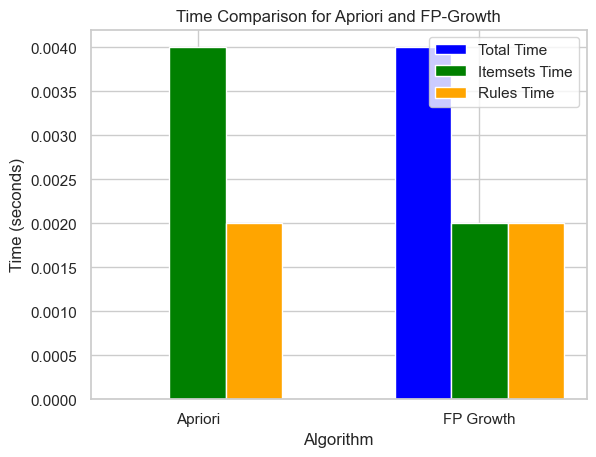
\includegraphics[width=0.7\textwidth]{Chapters/ch5/ch_5_bargraph.png}
    % \caption{Apriori graph}
    % \label{fig:example}
\end{figure}
\newpage
This graph shows how the total time for both processes (generating frequent itemsets and rule mining), just the time for frequent itemset generation, and just the time for association rule mining, differ from one another.


\subsection{Memory Usage:}

\begin{table}[htbp]
    \centering
    \rowcolors{1}{orange!20}{white}
    \renewcommand{\arraystretch}{1} % Adjust row height
    \begin{adjustbox}{max width=\textwidth}
    \begin{tabular}{|>{\columncolor{orange!50}}c|c|c|c|}
        \hline
        \rowcolor{orange!50}
        \textbf{Line\#} & \textbf{Memory Usage} & \textbf{Increment} & \textbf{Occurances} \\
        \hline
        41 & 142.1 MiB & 142.1 MiB & 1 \\
        42 &  &  & \\
        44 & 142.2 MiB & 0.1 MiB & 2 \\
        46 & 142.3 MiB & 0.0 MiB & 2 \\
        \hline
    \end{tabular}
    \end{adjustbox}
    \caption{Apriori}
    \label{tab:5x5_orange}
\end{table}

\begin{table}[htbp]
    \centering
    \rowcolors{1}{orange!20}{white}
    \renewcommand{\arraystretch}{1} % Adjust row height
    \begin{adjustbox}{max width=\textwidth}
    \begin{tabular}{|>{\columncolor{orange!50}}c|c|c|c|}
        \hline
        \rowcolor{orange!50}
        \textbf{Line\#} & \textbf{Memory Usage} & \textbf{Increment} & \textbf{Occurances} \\
        \hline
        53 & 142.3 MiB & 142.3 MiB & 1 \\
        54 &  &  & \\
        56 & 142.3 MiB & 0.0 MiB & 2 \\
        58 & 142.3 MiB & 0.0 MiB & 2 \\
        \hline
    \end{tabular}
    \end{adjustbox}
    \caption{Apriori}
    \label{tab:5x5_orange}
\end{table}


Both algorithms show minimal memory usage variations during their execution.
FP-Growth maintains a constant memory usage throughout its execution, indicating its ability to efficiently handle memory resources, especially for large datasets.
Apriori exhibits a slightly higher memory increment during the discovery of frequent itemsets, but the additional memory is modest and may not be a significant concern

% ----------------------------------------------------------------------------------------------------------------

\subsection{Summarized Differences:}

\begin{table}[htbp]
    \centering
    \rowcolors{2}{pink!20}{white}
    \begin{tabular}{|>{\bfseries\raggedright\arraybackslash}p{3cm}|>{\raggedright\arraybackslash}p{3cm}|>{\raggedright\arraybackslash}p{3cm}|>{\raggedright\arraybackslash}p{3cm}|}
        \hline
        \rowcolor{pink!80}
        {\textbf{Aspect}} & {\textbf{Apriori}} & {\textbf{FP-Growth}} & {\textbf{Empirical Evidence}} \\
        \hline
        Algorithmic Complexity & Generally, has higher algorithmic complexity, especially in the frequent itemset generation phase. & Lower algorithmic complexity due to a single-pass tree construction.& Apriori's complexity can lead to longer execution times, as seen in your data. \\
        Scalability & Tends to have scalability issues with large datasets and numerous itemsets. & More scalable, particularly for large datasets, as it requires fewer passes over the data. & FP-Growth may perform better as the dataset size increases, as suggested by your execution time results. \\
        Memory Requirements & Typically, higher memory requirements, especially when dealing with many transactions and items. & Lower memory requirements, especially for large datasets, as it constructs a compact FP-tree. & FP-Growth is expected to be more memory-efficient based on the provided data. \\
        Empirical Evidence & Apriori showed longer execution times, especially in the itemset generation phase. & FP-Growth demonstrated shorter execution times, indicating better performance. & The empirical evidence supports the idea that FP-Growth outperforms Apriori in terms of execution time. \\
        \hline
    \end{tabular}
    \caption{Table with 4 columns and 4 rows}
    \label{tab:4x4_sentences}
\end{table}
% \end{document}



% Chapter 1

\chapter{Tracking Patterns and Customer Behavior Analysis} % Main chapter title

\label{Chapter1} % For referencing the chapter elsewhere, use \ref{Chapter1} 

\lhead{Chapter 6. \emph{Tracking Patterns and Customer Behavior Analysis}} % This is for the header on each page - perhaps a shortened title

%----------------------------------------------------------------------------------------

\section{Creating Time-Series Data:}

 Time-series data is integral for tracking patterns and analyzing customer behavior evolution due to its ability to capture temporal nuances. By observing changes over time, businesses can uncover seasonal variations, identify trends, and forecast future behavior. This data-driven approach facilitates the detection of anomalies, adaptation of marketing strategies, and segmentation of customers based on temporal patterns. Utilizing time-series analysis improves decision-making, allowing businesses to make informed choices, allocate resources efficiently, and implement targeted campaigns, ultimately optimizing their strategies for dynamic customer preferences and market fluctuations.
\newline
 Hence, I utilized out existing ‘Date’ and ‘Time’ columns to create a ‘Timestamp’ feature for our dataset, which is evidently quite beneficial when conducting time-series analysis:


 % MAKE BLACK AND WHITE 
\begin{table}[htbp]
    \centering
    \rowcolors{1}{blue!20}{white}
    \begin{tabular}{|c|}
        \hline
        \rowcolor{blue!70}
        \textcolor{white}{\textbf{Timestamp Column:}} \\
        \hline
        \rowcolor{blue!50}
        0   2019-01-05 13:08:00\\
        1   2019-03-08 10:29:00 \\
        \rowcolor{blue!50}
        2   2019-03-03 13:23:00 \\
        3   2019-01-27 20:33:00 \\
        \rowcolor{blue!50}
        4   2019-02-08 10:37:00\\
        \hline
    \end{tabular}
    % \caption{Single-column table with alternating blue colors and a header}
    \label{tab:blue_table_with_header}
\end{table}

%----------------------------------------------------------------------------------------
\newpage
\section{Visualizations: }

\begin{figure}[h]
    \centering
    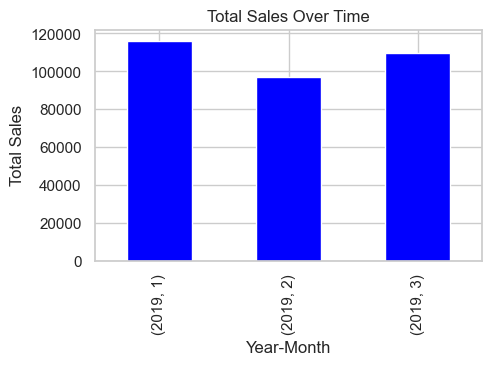
\includegraphics[width=0.7\textwidth]{Chapters/ch6/ch_6_bargraph_2.png}
    % \caption{Radar graph}
    % \label{fig:example}
\end{figure}
This chart depicts the total sales by year-month. As can be seen, February 2019 saw a fall in sales between January and March.
\newline 
\newline 
\begin{figure}[h]
    \centering
    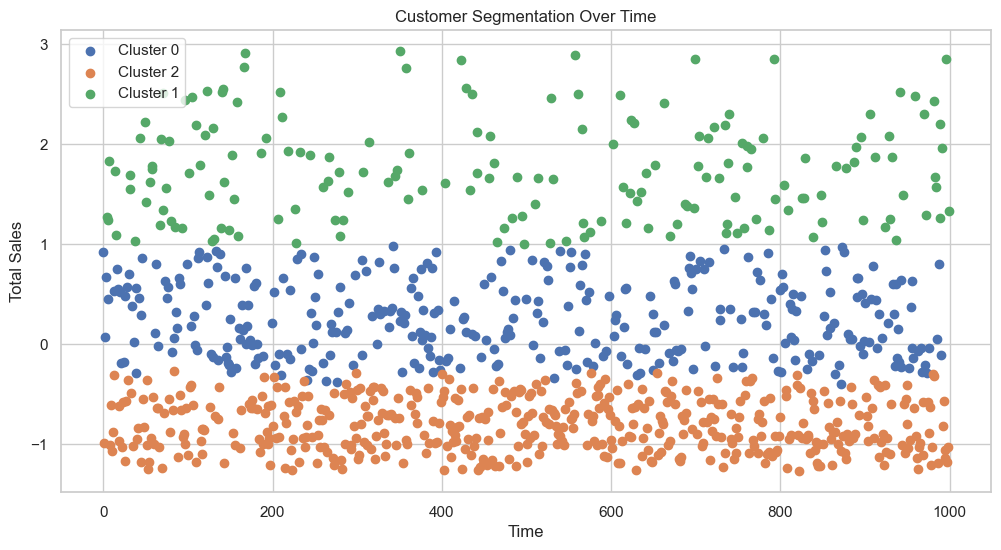
\includegraphics[width=0.7\textwidth]{Chapters/ch6/ch_6_scatterplot.png}
    % \caption{Radar graph}
    % \label{fig:example}
\end{figure}

Using clustering, I was able to visualize customer segmentation over time.

\newpage 
\subsection{Seasonal Decompose Graphs:}

\begin{figure}[h]
    \centering
    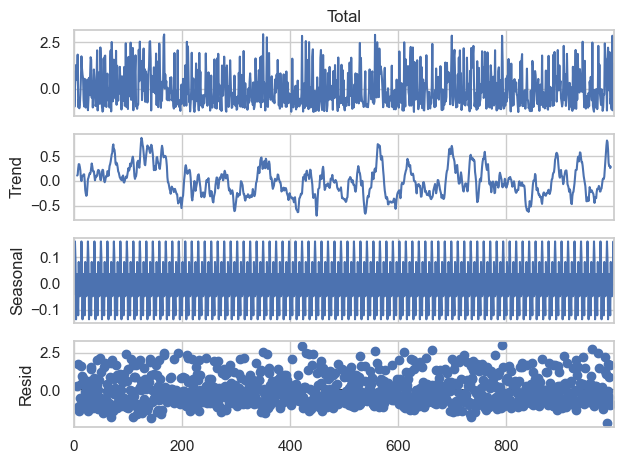
\includegraphics[width=0.7\textwidth]{Chapters/ch6/ch_6_decompose_graph.png}
    % \caption{Radar graph}
    % \label{fig:example}
\end{figure}

Using the \verb|seasonal_decompose| function from statsmodels.tsa, I decomposed a time series into three components: trend, seasonality, and residual. The model is set to 'additive', which means the components are added together. The period is set to 12, indicating a seasonal pattern with a period of 12-time units. 

\begin{itemize}
    \item Observed Component (First Graph): 
    \newline 
    The top scatter plot represents the original time series, which is the observed component. 
As can be seen in the plot, the dense values with high variance suggest that the original time series has fluctuations, noise, or irregular patterns.
    
    \item Trend Component (Second Graph):
    \newline 
    Sets a minimum threshold for the chosen metric. Rules with a confidence value above this threshold will be considered.

    \item Seasonal Component (Third Graph):
    \newline 
    This graph captures the periodic patterns or seasonality in the data, showing how the data varies with a fixed interval (e.g., season). 

    \item Residual Component (Fourth Graph):
    \newline
    This represents the remaining variability after removing the trend and seasonal components. It's essentially the difference between the observed data and the predicted values from the trend and seasonal components. The dense scatter plot suggests that the residuals still contain some variability or noise that is not explained by the trend and seasonal components.
    
\end{itemize}



\subsection{Predictive Modeling using ARIMA: }
ARIMA stands for AutoRegressive Integrated Moving Average. It is a popular time series forecasting model that combines three components: AutoRegressive (AR), Integrated (I), and Moving Average (MA).

\subsubsection{How is it beneficial here? }
ARIMA helps identify and model patterns in the time series data, including seasonality, trends, and cyclical behaviors. It captures historical patterns to make predictions about future values.
\newline 
\newline 
Forecasting Customer Behavior: By applying ARIMA to historical customer behavior data (e.g., sales over time), the model can provide forecasts for future behavior. This can be valuable for planning marketing strategies, inventory management, and overall business decision-making.
\newline 
\newline 
Understanding Trends: The trend component of the ARIMA model helps in understanding the overall direction of the time series. This can be useful in identifying long-term trends in customer behavior.
\newline 
\newline 
ARIMA models, however, assume that the underlying patterns in the data are linear and stationary. For more complex and dynamic patterns, other time series models or machine learning approaches may be considered.


\subsubsection{Applying the model:}
ARIMA(df5['Total'], order=(1, 1, 1)): This initializes an ARIMA model using the ARIMA class.
order=(1, 1, 1) specifies the order of the ARIMA model. Here, (1, 1, 1) means:

\begin{itemize}
    \item p=1: One autoregressive term. It models the relationship between the current value and its immediate previous value (lag 1).
    
    \item d=1: One differencing. It indicates that the time series is differenced once to achieve stationarity. Differencing involves subtracting the previous value from the current value.

    \item q=1: One moving average term. It models the dependency between the current value and the residual error from the lagged moving average terms.
\end{itemize}

model.fit(): This fits the ARIMA model to the provided time series data (df5['Total']).
\verb|result.get_forecast(steps=forecast_steps)|: This generates forecasts for the next \verb|forecast_steps| time points using the fitted ARIMA model.
\verb|predicted_mean|: This extracts the predicted mean values from the forecast result. The mean values represent the point estimates of the forecast.


\subsubsection{Prediction and analysis}

\begin{figure}[h]
    \centering
    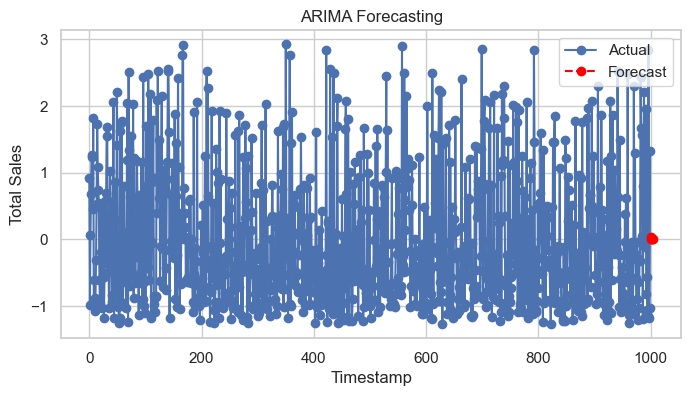
\includegraphics[width=0.7\textwidth]{Chapters/ch6/ch_6_pred_and_analysis.png}
    % \caption{Radar graph}
    % \label{fig:example}
\end{figure}

The dense distribution of blue points represents the actual "Total" sales values over time. The constant variation suggests that the sales data exhibit fluctuations or variability.
\newline 

The sparse presence of red points (forecast) at the end of the x-axis indicates the predicted "Total" sales values for the next 5 time points. The small size of the red dots suggests that the model is forecasting relatively low variations or changes in sales over this short-term forecast horizon. Hence, there seems to be a relatively stable or slowly changing trend in future sales.
\newline 
% \newline 
The sparse and concentrated nature of the red points might also suggest a high level of confidence in the forecast, as the model is projecting a narrow range of potential outcomes.
\newline 
% \newline
From all this we may conclude that there won’t be much change in customer behavior soon.

\subsection{Feature Engineering to calculate and visualize Rolling Mean:}
\newpage 
\subsubsection{The visualization:}
\begin{figure}[h]
    \centering
    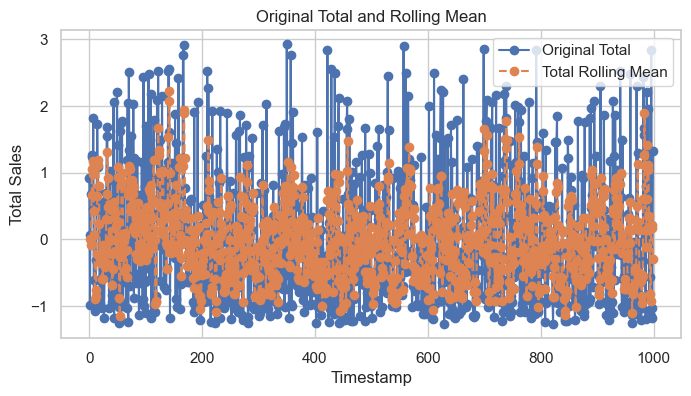
\includegraphics[width=0.7\textwidth]{Chapters/ch6/ch_6_rolling_mean.png}
    % \caption{Radar graph}
    % \label{fig:example}
\end{figure}

\subsubsection{How the graph works: }
The purpose of calculating the rolling mean is to smooth out short-term fluctuations or noise in your data and highlight longer-term trends. In this case, we are using it to provide a clearer picture of how the "Total" sales values are evolving over time. We’re using a rolling window of size 3. A rolling window refers to a fixed-size subset of consecutive data points that "rolls" or moves through the dataset as you analyze it. This helps in revealing trends and patterns.

\subsubsection{Analyzing the visualization}
The dense blue (Original Total) that can be seen throughout the graph, indicates frequent fluctuations or variations in the sales values. This could be due to regular transactions or short-term patterns in customer behavior. \newline 
In contrast, the orange points (Total Rolling Mean) are denser at the bottom half of the chart. Thus, the rolling mean is consistently lower than the actual sales value. This represents a downward trend or a smoothing effect that levels out short-term spikes or peaks in the original data. Hence, there are periods of lower sales that are being averaged out.
\newline 
Based on all this, we can conclude that there are frequent fluctuations in total sales, which are potentially being influenced by daily transactions or short-term trends. 

%----------------------------------------------------------------------------------------

% Chapter 1

\chapter{Sequential Pattern Mining} % Main chapter title

\label{Chapter1} % For referencing the chapter elsewhere, use \ref{Chapter1} 

\lhead{Chapter 7. \emph{Sequential Pattern Mining}} % This is for the header on each page - perhaps a shortened title

%----------------------------------------------------------------------------------------

\section{Relevance to this project }

Sequential Pattern Mining is a data mining technique that aims to discover patterns in sequential data, such as sequences of events or itemsets in a transactional dataset. In our project, sequential pattern mining can reveal interesting associations and orderings of itemsets across transactions and time periods. It may help identify frequent sequences of itemsets in the dataset. Patterns can reveal customer buying behavior, such as common sequences of products purchased together over time. 
\newline 
The goal of sequential pattern mining is to discover frequent sequences of items within a dataset. In the context of retail or supermarket sales, this could reveal common patterns of items that customers tend to purchase together, providing insights into customer behavior over time. 
\newline 
I decided to use a support value of 0.1 for all algorithms that I used.

\section{How is this different from using Apriori or FP Growth?}

\begin{table}[htbp]
    \centering
    \begin{adjustbox}{max width=\textwidth}
        \rowcolors{1}{green!20}{white}
        \begin{tabular}{|>{\columncolor{green!50}}c|c|c|}
            \hline
            \rowcolor{green!70}
            \textbf{Feature} & \textbf{Sequential Pattern Mining} & \textbf{Apriori Algorithm} \\
            \hline
            Focus & Temporal order of events or itemsets & Frequent itemsets without order concern \\
            Goal & Discover frequent sequences of items & Discover frequent sets of items \\
            Order Sensitivity & Emphasizes order sensitivity & Not inherently order-sensitive \\
            Data Structure & Utilizes sequence databases or similar & Utilizes itemsets and transaction data \\
            Use Cases & Analyzing time-ordered data (e.g., transactions over time) & Finding associations in static datasets \\
            Example Use Case & Identifying common sequences of products purchased over time & Identifying frequent sets of products irrespective of order\\
            \hline
        \end{tabular}
    \end{adjustbox}
    % \caption{Comparison of Sequential Pattern Mining and Apriori Algorithm}
    \label{tab:sequential_apriori_comparison}
\end{table}

\section{PrefixSpan:}

\subsection{How does it work?}
PrefixSpan employs a depth-first search strategy to explore the space of possible sequential patterns. It uses a divide-and-conquer approach to efficiently find frequent sequences without generating all possible combinations.
\newline 
\newline
The algorithm starts by considering each unique item in the dataset as a prefix and explores its extensions. For each prefix, it identifies the occurrences of that prefix in the dataset and extends it to find longer sequential patterns.
\newline
\newline
The recursion is a key feature of PrefixSpan. For each identified prefix, the algorithm recursively projects the remaining sequences and searches for frequent patterns in the projected sequences. This recursive approach allows PrefixSpan to efficiently discover sequential patterns of varying lengths.


\subsection{Applying it via code:} 
I made use of the list of lists I had already computed in a previous task, as the input to this algorithm. Following is the main line in which I applied PrefixSpan:
\begin{lstlisting}[language=Python, frame=none]
patterns = PrefixSpan(transactions_list).frequent(0.1, closed=True)
\end{lstlisting}
The frequent method is applied to the PrefixSpan instance. It discovers frequent sequential patterns in the dataset based on a minimum support threshold of 0.1 (10\%). The closed=True parameter indicates that closed sequential patterns should be included in the results.

The discovered patterns are then iterated over. This helps inspect and analyze the frequent sequential patterns in your dataset.

\subsection{Result and Analysis:}
\newline
\newline 
\textbf{Output}
(1, ['Health', 'beauty'])
\newline 
(1, ['Home', 'lifestyle'])
\newline 
(1, ['Sports', 'travel'])
\newline 
(1, ['Electronic accessories'])
\newline 
(1, ['Food', 'beverages'])
\newline
(1, ['Fashion accessories'])
\newline 
\newline 
These patterns signify sequences of itemsets that frequently occur together in transactions. The support value indicates how often each sequence appears in the dataset. Since all support values are 1 here, it indicates that each sequence occurred in exactly one transaction, meaning they are not very common or frequent.

%----------------------------------------------------------------------------------------

\section{GSP: Generalized Sequential Patterns:}

\subsection{How does it work?}
GSP employs a sliding window approach to traverse the sequence of events systematically. This involves moving a fixed-size window or 'frame' across a sequence of data points, analyzing the data within the window at each position. The window slides through the sequence, typically one step at a time, capturing a subset of the data at each step.
\newline 
GSP employs a breadth-first search strategy to explore the space of potential sequential patterns. GSP initially identifies frequent individual items and progressively extends them to discover longer patterns. The algorithm uses a candidate generation and pruning mechanism to efficiently identify patterns that meet the minimum support threshold. GSP iterates through the sequence, adjusting the size of the sliding window dynamically to capture patterns of varying lengths.

\subsection{Applying it via code:}
In the implementation of GSP, I utilized the seqmining library to discover frequent sequential patterns. The freq_seq_enum method is applied to find sequences with a minimum support threshold of 0.1 (10\%). The results are then iterated over, allowing for inspection and analysis of the frequent sequential patterns in the dataset.

\subsection{Result and Analysis:}
\textbf{Output:}
\newline
(('Food',), 1)
\newline
(('Health',), 1)
\newline
(('travel',), 1)
\newline
(('Fashion accessories',), 1)
\newline
(('Health', 'beauty'), 1)
\newline
(('Food', 'beverages'), 1)
\newline
(('Home',), 1)
\newline
(('lifestyle',), 1)
\newline
(('Electronic accessories',), 1)
\newline
(('beverages',), 1)
\newline
(('Sports',), 1)
\newline
(('Sports', 'travel'), 1)
\newline
(('beauty',), 1)
\newline
(('Home', 'lifestyle'), 1)
\newline 
\newline 
The support count of 1 for each pattern indicates that the identified sequential patterns occur infrequently in the dataset. This might suggest that customers exhibit varied and unique purchasing patterns, and there isn't a dominant sequential pattern that applies to a large portion of the dataset.


\section{Eclat Algorithm (Equivalence Class Transformation):}

\subsection{How does it work?}
Eclat utilizes a vertical data representation, where each column corresponds to a unique item, and each row represents a transaction. It focuses on finding frequent itemsets by constructing equivalence classes for each item. Equivalence refers to a state of being equal or having the same value. These equivalence classes consist of sets of transactions containing the respective item. Eclat then intersects these equivalence classes to discover frequent itemsets of larger sizes. Its recursive approach ensures the discovery of progressively longer patterns. The vertical data representation and intersection-based technique contribute to Eclat's efficiency in mining frequent itemsets in datasets.

\subsection{Applying it via code:}
For Eclat, I employed the pyECLAT library, creating a DataFrame from the list of transactions. The ECLAT class is then used to find frequent itemsets with a minimum support of 0.1. The discovered itemsets are iterated over, facilitating an examination of the frequent itemsets in the dataset.

\subsection{Result and Analysis:}
\textbf{Output:}
'beverages': [4], 'Food': [4], 'Sports': [2], 'lifestyle': [1], 'Home': [1], 'Electronic accessories': [3], 'beauty': [0], 'Fashion accessories': [5], 'travel': [2], 'Health': [0], 'beverages & Food': [4], 'Sports & travel': [2], 'lifestyle & Home': [1], 'beauty & Health': [0]}
{'beverages': 0.16666666666666666, 'Food': 0.16666666666666666, 'Sports': 0.16666666666666666, 'lifestyle': 0.16666666666666666, 'Home': 0.16666666666666666, 'Electronic accessories': 0.16666666666666666, 'beauty': 0.16666666666666666, 'Fashion accessories': 0.16666666666666666, 'travel': 0.16666666666666666, 'Health': 0.16666666666666666, 'beverages & Food': 0.16666666666666666, 'Sports & travel': 0.16666666666666666, 'lifestyle & Home': 0.16666666666666666, 'beauty & Health': 0.16666666666666666}
\newline 
\newline 
The diversity in item combinations and the uniform distribution of relative support values across different items imply that customers exhibit varied purchasing behaviors. There isn't a dominant sequential pattern or a specific set of items that consistently appear together in the dataset.


% -------------------------------------------------------------------------------------------
\section{Summarization of Key Differences}

\begin{table}[htbp]
    \centering
    \begin{adjustbox}{max width=\textwidth}
    \rowcolors{1}{pink!20}{white}
    \begin{tabular}{|>{\columncolor{pink!50}}c|c|c|}
        \hline
        \rowcolor{pink!70}
        \textbf{Algorithm} & \textbf{Output (Sample)} & \textbf{Key Differences and Inferences} \\
        \hline
        PrefixSpan & ('Health', 'beauty')('Food', 'beverages')
        & Occurrence is infrequent, suggesting unique purchasing patterns; no dominant sequential pattern. \\
        GSP & ('Food')('Sports', 'travel') & Patterns occur infrequently; no clear dominant sequential pattern in the dataset. \\
        Eclat & {'beverages': [4], 'Food': [4], 'Sports': [2]}
{'beverages': 0.17, 'Food': 0.17, 'Sports': 0.17}
& Diversity in item combinations, uniform support distribution; no dominant sequential pattern identified. \\
        \hline
    \end{tabular}
    \end{adjustbox}
    % \caption{4 by 3 Table with Pink Alternating Row Colors}
    \label{tab:pink_table}
\end{table}

% Chapter 1

\chapter{Clustering} % Main chapter title

\label{Chapter8} % For referencing the chapter elsewhere, use \ref{Chapter1} 

\lhead{Chapter 8. \emph{Clustering}} % This is for the header on each page - perhaps a shortened title

%----------------------------------------------------------------------------------------

\section{Importance of feature selection }

 Feature selection in the context of clustering refers to the process of choosing a subset of relevant features from the original set of features in a dataset before applying a clustering algorithm. This selection is performed to enhance the quality of clustering results and improve the efficiency of the clustering process.
 
 \section{Selection of features and reasoning}
 I selected: 'Unit price', 'Quantity', 'Tax 5\%', 'Total', 'cogs', 'gross income' and 'Rating'. 
 \newline 
Features like 'Unit price', 'Quantity', and 'Total', are likely to capture essential aspects of customer transactions. 'Rating' could provide insights into customer satisfaction. In addition to this, all the features I chose are commonly associated with sales transactions and customer behavior in retail. An alternative could’ve been employing some feature selection technique, like PCA. However, for this specific task, I chose to deal manually with feature selection.
\newline 
For all the plots, I’ve used the features ‘Total’ and ‘Rating’ for the axes.


\section{Why a standardized dataset is required:}
Standardization deals with issues related to scale disparities among features, which can significantly impact the performance of distance-based algorithms like KMeans. By transforming data to a common scale, standardization prevents biases toward features with larger magnitudes, enhances convergence, and facilitates meaningful comparisons. It also promotes model interpretability by ensuring that cluster centroids represent average values across features consistently. 

\section{Applying Clustering}
\subsection{Kmeans}
K-Means is a popular partitioning algorithm that divides a dataset into K clusters. It aims to minimize the sum of squared distances between data points and the centroid of their assigned cluster. It assigns each data point to the cluster with the nearest centroid.


\begin{table}[htbp]
    \centering
    \begin{adjustbox}{max width=\textwidth}
    \rowcolors{1}{green!20}{white}
    \begin{tabular}{|>{\columncolor{green!50}}c|c|}
        \hline
        \rowcolor{green!70}
        \textbf{Metric Name} & \textbf{Score} \\
        \hline
        Inertia (K-Means) & 2705.273033683108 \\
        Silhouette Score & 0.3037813725498845 \\
        Davies-Bouldin Index  & 1.1812055382786706 \\
        Calinski-Harabasz Index  & 791.3882872643744 \\
        \hline
    \end{tabular}
    \end{adjustbox}
    % \caption{5 by 2 Table with Light Green Alternating Row Colors}
    \label{tab:green_table}
\end{table}

The numbers indicate a moderate level of compactness (Inertia: 2705.27) and well-defined clusters, as indicated by the Silhouette Score (0.30), Davies-Bouldin Index (1.18), and Calinski-Harabasz Index (791.39). These metrics collectively suggest that the chosen number of clusters (3) is appropriate for grouping customers based on their purchase history. The clusters exhibit reasonable separation and distinctiveness, providing valuable insights for customer segmentation.

\begin{figure}[h]
    \centering
    \begin{minipage}{0.45\textwidth}
        \centering
        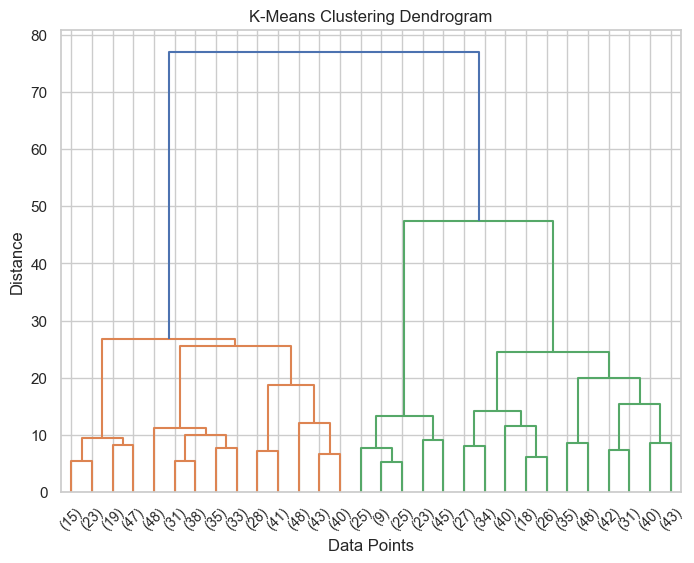
\includegraphics[width=\linewidth]{Chapters/ch8/ch_8_kmeans_dendo.png}
        \caption{Dendrogram}
        \label{fig:dendrogram}
    \end{minipage}\hfill
    \begin{minipage}{0.45\textwidth}
        \centering
        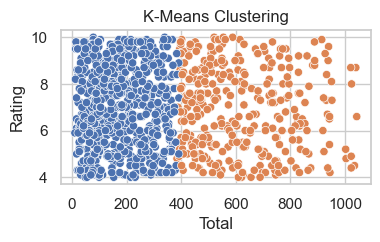
\includegraphics[width=\linewidth]{Chapters/ch8/ch_8_kmeans_scatter.png}
        \caption{Scatterplot}
        \label{fig:scatterplot}
    \end{minipage}
\end{figure}



% ----------------------------------------------------------------------------------------


\subsection{K-Median}
Like K-Means, K-Median is a partitioning algorithm that seeks to minimize the sum of absolute differences (medians) between data points and the centroid of their assigned cluster. K-Median is more robust to outliers compared to K-Means.

\begin{figure}[h]
    \centering
    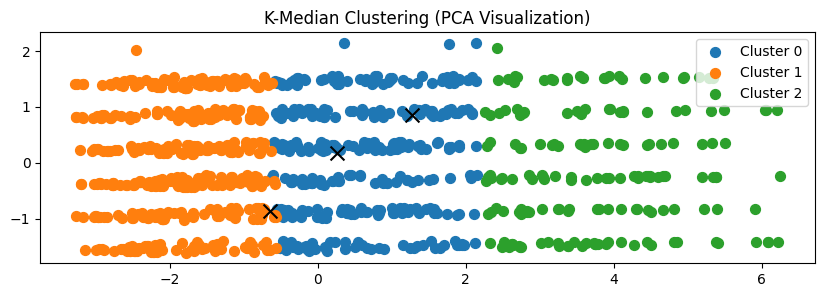
\includegraphics[width=0.7\textwidth]{Chapters/ch8/ch_8_kmedian_scatter (2).png}
    \caption{Scatter plot}
    % \label{fig:example}
\end{figure}

\subsection{ARI and NMI}
\begin{table}[htbp]
    \centering
    \begin{adjustbox}{max width=\textwidth} % Fit the table to the page width
        \rowcolors{1}{green!20}{white} % Alternate row colors starting from the second row
        \rowcolors{2}{green!30}{white} % Slightly darker header row
        \begin{tabular}{|>{\columncolor{green!50}}c|c|}
            \hline
            \rowcolor{green!50} % Slightly darker header row color
            \textbf{Metric} & \textbf{Score} \\
            \hline
            Adjusted Rand Index (ARI) & 0.5451 \\
            Normalized Mutual Information (NMI) & 0.5859 \\
            \hline
        \end{tabular}
    \end{adjustbox}
    % \caption{3 x 2 Table with alternating light green rows and a slightly darker green header}
    \label{tab:3x2_table}
\end{table}
The Adjusted Rand Index (ARI) measures the similarity between clusters obtained by different algorithms. A score of 0.5451 indicates a moderate agreement between K-Means and Agglomerative Clustering.
\newline
Normalized Mutual Information (NMI) measures the mutual dependence between clusters. The score of 0.5859 suggests a reasonable degree of similarity between the two clustering methods.

% \newpage
% \subsection{results}
The similarity in results between K-Means and Agglomerative Clustering suggests that both algorithms capture similar patterns in the data. 
\begin{figure}[h]
    \centering
    \begin{minipage}{0.45\textwidth}
        \centering
        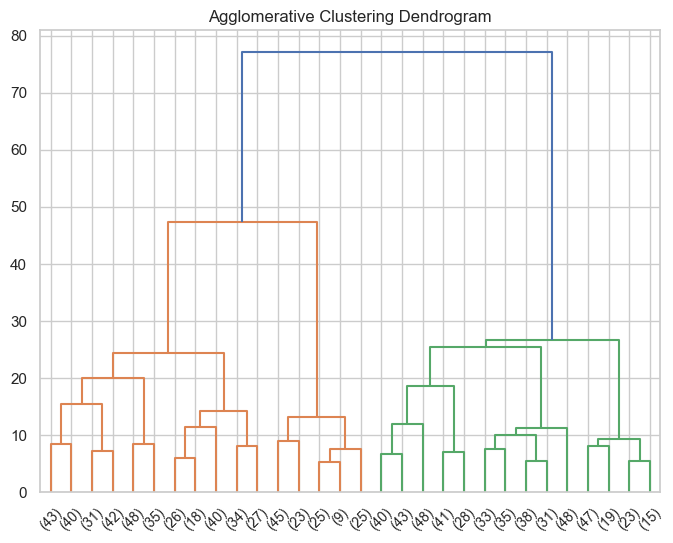
\includegraphics[width=\linewidth]{Chapters/ch8/ch_8_agglo_dendo.png}
        \caption{Dendrogram}
        \label{fig:dendrogram}
    \end{minipage}\hfill
    \begin{minipage}{0.45\textwidth}
        \centering
        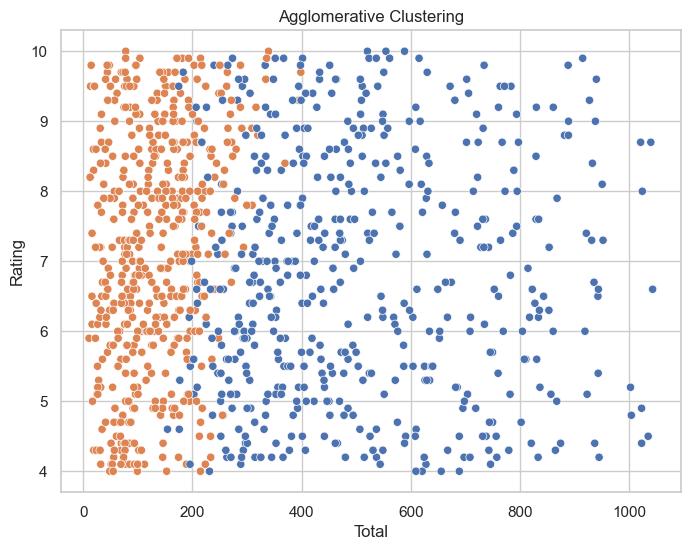
\includegraphics[width=\linewidth]{Chapters/ch8/ch_8_agglo_scatter.png}
        \caption{Scatterplot}
        \label{fig:scatterplot}
    \end{minipage}
\end{figure}



% -------------------------------------------------------------------------------------------------------------
\subsection{DBSCAN:}

\begin{table}[htbp]
    \centering
    \begin{adjustbox}{max width=\textwidth} % Fit the table to the page width
        \rowcolors{1}{green!20}{white} % Alternate row colors starting from the second row
        \rowcolors{2}{green!30}{white} % Slightly darker header row
        \begin{tabular}{|>{\columncolor{green!50}}c|c|}
            \hline
            \rowcolor{green!50} % Slightly darker header row color
            \textbf{Metric} & \textbf{Score} \\
            \hline
            Silhouette Score (DBSCAN)  & 0.12528450383737091 \\
            Davies-Bouldin Index (DBSCAN)  & 1.5543217530912334 \\
            Number of Clusters (DBSCAN) & 23 \\
            \hline
        \end{tabular}
    \end{adjustbox}
    % \caption{3 x 2 Table with alternating light green rows and a slightly darker green header}
    \label{tab:3x2_table}
\end{table}

In applying DBSCAN to cluster customers based on purchase history, the algorithm identified 23 clusters. However, the negative Silhouette Score of approximately -0.125 indicates potential overlap between clusters, while the Davies-Bouldin Index of around 1.55 suggests moderate separation. These results may be indicative of the algorithm's sensitivity to data density and its tendency to partition the dataset into numerous, potentially small, dense regions. 

\begin{figure}[h]
    \centering
    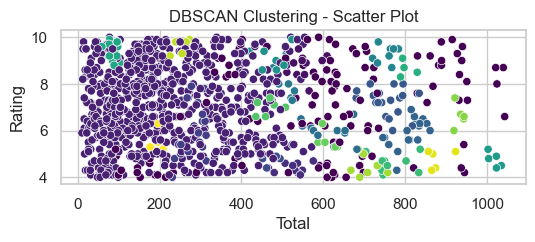
\includegraphics[width=0.7\textwidth]{Chapters/ch8/ch_8_dbscan_scatter.png}
    \caption{scatter plot}
    % \label{fig:examle}
\end{figure}

% \section{Mean Shift}
% \begin{figure}[h]
%     \centering
%     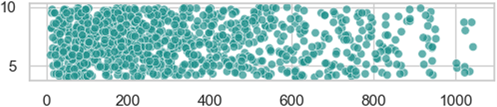
\includegraphics[width=0.7\textwidth]{Chapters/ch8/scatterplot_5.png}
%     % \caption{Radar graph}
%     % \label{fig:example}
% \end{figure}
% The single-cluster prediction by Mean Shift indicates its unsuitability for the task at hand. Mean Shift's sensitivity to overall data density and homogeneity may lead to oversimplification and a failure to discern distinct clusters in the presence of irregularly shaped or non-convex structures.



% ------------------------------------------------------------------------------------------

% Chapter 9

\chapter{Classification} % Main chapter title

\label{Chapter9} % For referencing the chapter elsewhere, use \ref{Chapter1} 

Since most preprocessing required for classification here had already been performed in the first task of the project, I did not feel the need to conduct it again and simply re-used the dataset at the standardization stage. So, this is a sample of the DataFrame I started working with:

\begin{figure}[h]
    \centering
    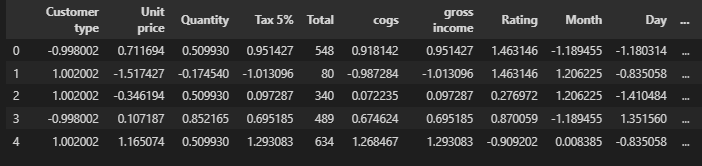
\includegraphics[width=1\textwidth]{Chapters/ch9/data_1.png}
    % \caption{This is an example image.}
    % \label{fig:example}
\end{figure}

\lhead{Chapter 9. \emph{Classification}} % This is for the header on each page - perhaps a shortened title

%----------------------------------------------------------------------------------------

\section{Choosing the Target Variable:}

 In the context of our problem (Customer Segmentation), the target variable was a choice between 2 features. Although other features could also be utilized, these 2 features seemed the best for performing customer segmentation. The 2 features are ‘Total’ and ‘Customer type’. 
 \newline 
 I chose ‘Total’ due to its direct relevance to overall customer spending. It encapsulates the comprehensive financial transaction for each customer, making it a meaningful and practical variable for segmentation. The choice is justified by the potential predictive power of variations in spending patterns, the business relevance of understanding different customer segments, and the ability to employ classification metrics for model evaluation. Furthermore, the interpretability of 'Total' spending segments enhances the practical impact on business decision-making, aligning with the overarching goal of gaining actionable insights into customer behavior.
 \newline
 ‘Customer type’, on the other hand, enables the model to differentiate between distinct customer types, such as "Member" and "Normal," offering valuable information for targeted marketing strategies, loyalty programs, and operational decision-making. Predicting customer types can aid in customer retention efforts and enhance the overall customer experience by tailoring services to the specific needs and expectations of different segments. 
 \newline 
 Hence, from a business as well as a technical perspective (applying models), both features seem to make a lot of sense as the target variable. As I mentioned before, there are other features that could be used for this task as well. These include Product line, Payment Method, and Quantity. For customer segmentation specifically however, I felt ‘Total’ and ‘Customer type’ made more sense.
 \newline
 I chose ‘Total’ from these two because I wanted to explore the concept and application of binning. As ‘Total’ is a continuous feature and ‘Customer type’ is categorical.
\newline 
By this point, I had cleaned, encoded, and standardized the data. However, binning was required before splitting the data, since my chosen target variable was ‘Total’, and this is a continuous feature in the dataset.

\section{Binning:}

\subsection{The concept of binning:}
Binning, also known as discretization, is a data preprocessing technique commonly used in data analysis and machine learning to handle numerical data. The general logic behind binning is to simplify the data and make it more manageable, especially when dealing with continuous variables. This process involves grouping a range of continuous or numerical data points into a smaller number of discrete "bins" or intervals.

\subsection{Choosing an ideal number of bins:}
For this step, I decided to use various rules which help indicate the ideal value for bins to use.

\subsubsection{Square Root Rule:}
This is a simple method that calculates the number of bins by taking the square root of the total number of data points in the dataset. The formula is usually given as sqrt(n), where 'n' is the number of data points. It is easy to apply and works well for datasets of various sizes. It helps in preventing the creation of too many or too few bins.

\subsubsection{Sturges’ Formula:}
\begin{equation}
k = 1 + \log^2(N)
\end{equation}
where:
\begin{itemize}
\item k is the number of bins.
\item N is the number of data points.
\end{itemize}

This formula assumes that the data follows a normal distribution. It is widely used and is suitable for datasets with a normal distribution. However, it may not perform well for datasets with outliers or non-normal distributions.

\subsubsection{Scott’s Rule:}
\begin{equation}
3.5 * (S.D.) * (n^(-1/3))
\end{equation}
where:
\begin{itemize}
\item h is the bin width.
\item N is the number of data points.
\end{itemize}

This rule considers the variability of the data.
It is robust and performs well for datasets with varying degrees of variability. It adapts to the distribution of the data and is less sensitive to outliers.

\subsubsection{Freedman-Diaconis Rule:}
\begin{equation}
2 * IQR * (n^(-1/3))
\end{equation}
where:
\begin{itemize}
\item h is the bin width.
\item IQR is the interquartile range.
\item N is the number of data points.
\end{itemize}
This rule is particularly useful when dealing with datasets with outliers. It adjusts the bin width based on the spread of the data, making it less sensitive to extreme values.

\subsubsection{Doane’s Formula:}
\begin{equation}
    1 + log2(n) + log2(1 + |g1|/sigma_g1)
\end{equation}
where:
\begin{itemize}
\item k is the number of bins.
\item N is the number of data points.
\item g1 is the skewness of the data.
\item sigma(g1) is the standard error of the skewness.
\end{itemize}

This Formula is an extension of Sturges' Formula that also considers the skewness of the data. It is suitable for datasets with non-normal distributions and can provide a more accurate estimate of the number of bins when skewness is present.

\subsubsection{Results}
Here are all the results summarized:
\begin{table}[htbp]
    \centering
    \begin{adjustbox}{max width=\textwidth} % Fit the table to the page width
        \rowcolors{1}{green!20}{white} % Alternate row colors starting from the second row
        \rowcolors{2}{green!30}{white} % Slightly darker header row
        \begin{tabular}{|>{\columncolor{green!50}}c|c|}
            \hline
            \rowcolor{green!50} % Slightly darker header row color
            \textbf{Method} & \textbf{Number of Bins} \\
            \hline
            Square Root Rule  & 31 \\
            Sturges' Formula  & 11 \\
            Scott's Rule & 11 \\
            Freedman-Diaconis Rule & 14 \\
            Doane's Formula & 13 \\
            \hline
        \end{tabular}
    \end{adjustbox}
    % \caption{3 x 2 Table with alternating light green rows and a slightly darker green header}
    \label{tab:3x2_table}
\end{table}


Thus, from these results, the bin values were tending towards a value around 12. However, upon using such several bins, I faced issues. Hence, I went back to conduct further analysis:


\begin{figure}[h]
    \centering
    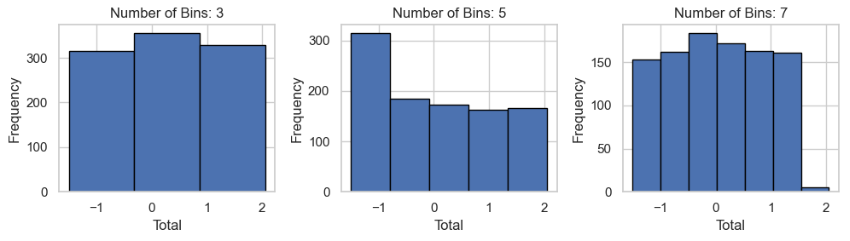
\includegraphics[width=0.7\textwidth]{Chapters/ch9/binning-1.png}
    % \caption{Radar graph}
    % \label{fig:example}
\end{figure}
\begin{figure}[h]
    \centering
    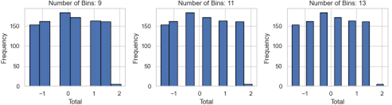
\includegraphics[width=0.7\textwidth]{Chapters/ch9/bar_chart_2.png}
    % \caption{Radar graph}
    % \label{fig:example}
\end{figure}

As can be seen from these graphs, a higher value for the bins seems to form a sparser distribution. Thus, we might want to use a lower number of bins.

\begin{figure}[h]
    \centering
    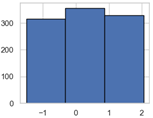
\includegraphics[width=0.2\textwidth]{Chapters/ch9/bar_chart_3.png}
    % \caption{Radar graph}
    % \label{fig:example}
\end{figure}
Judging from this, I decided to choose the number of bins to be 3, which seemed to be the ideal value as can be seen by this graph. All 3 bars, each representing a discrete ‘Total’ value, have an almost equal number of frequencies in our dataset. 


\subsection{Deciding on the bin edges:}
Once I decided how many bins to use, the next step was figuring out what values were to be assigned to these bins. Let me explain. I chose the number of bins for ‘Total’ to be 3. Which means that the ‘Total’ column will be discretized into 3 categories. But on what basis? How will we decide what value the original ‘Total’ goes into which bin? For this, I explored our data some more:
\newline
\newline
As can be seen below, the count of the discrete values present in ‘Total’ is 546:
\newline
Total
\newline
125    6
\newline
175    6
\newline
      ..
\newline
721    1
\newline
149    1
\newline
649    1
\newline
Name: count, Length: 546, dtype: int64
\newline
Also note, the Variance of the column ‘Total’ is 60457.8.
\newline 
\newline 
These values have given us an idea about the spread of the column ‘Total’. To understand this spread more, its evenness and unevenness, I used the following visualizations:
\begin{figure}[h]
    \centering
    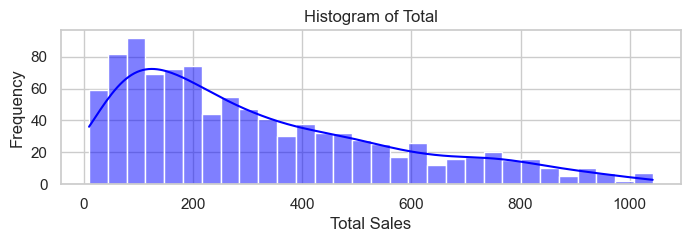
\includegraphics[width=0.5\textwidth]{Chapters/ch9/ch_9_hist.png}
    % \caption{Radar graph}
    % \label{fig:example}
\end{figure}
\begin{figure}[h]
    \centering
    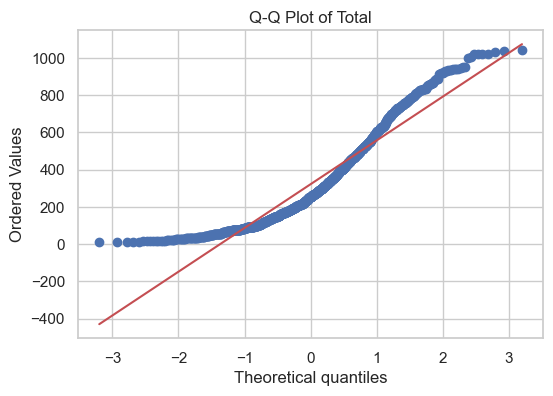
\includegraphics[width=0.5\textwidth]{Chapters/ch9/ch_9_linechart.png}
    % \caption{Radar graph}
    % \label{fig:example}
\end{figure}
As can be seen here, the blue line (actual values) does not follow a straight line, meaning the ‘Total’ column is not normally distributed. The points deviate from the line, especially towards the tails, which indicates a departure from normality. The points curving upwards and downwards suggest skewness or light/heavy-tailed distribution.
\newline
\newline
I made use of the ‘Quantile’ method to calculate the bin edges.  This method allows us to identify the values corresponding to specific percentiles within the distribution of the 'Total' column. I computed the 33rd and 66th percentiles, and the resulting values are utilized as reference points for defining the bin edges. Following is the code for this process:

\begin{lstlisting}[language=Python, frame=none]
percentile\_33 = df\_classif['Target'].quantile(0.33) 
percentile\_66 = df\_classif['Target'].quantile(0.66) 
bin\_edges = [df\_classif['Target'].min()
, percentile\_33, percentile\_66,df\_classif['Target'].max()] 
Bin Edges: 
[10, 163.0, 381.68000000000006, 1042]
\end{lstlisting}

\subsection{Applying binning:}
The last step before applying binning was to set the bin labels. I decided to set these to Low, Medium, and High. Since we’re applying binning on our ‘Total’ feature, which represents the total bill for each transaction, these labels seem to be good choices to categorize customer behavior.
\newline 
\newline
After this, I applied binning using our decided labels, edges, and number of bins:
\begin{lstlisting}[language=Python, frame=none]
df_classif['Total_bins'] = pd.cut(df_classif[column_name], bins=bin_edges, labels=bin_labels, include_lowest=True)
\end{lstlisting}
\newline 
\newline 
I made use of the powerful Pandas function ‘pd.cut’ to discretize the continuous feature ‘Total’. The first 3 parameters of the function are self-explanatory. The fourth parameter (include\_lowest) determines whether the leftmost edge of the bins should be considered as a valid bin edge or not. I’ve set this to true.
\newline 
\newline 
Here is the result following binning:
\newline 
0        High
\newline 
1         Low
\newline 
2      Medium
\newline 
3        High
\newline 
4        High
\newline 
        ...
\newline 
995       Low
\newline 
996      High
\newline 
997       Low
\newline
998       Low
\newline 
999      High
\newline 
Name: Total, Length: 1000, dtype: category
\newline 
Categories (3, object): ['Low' < 'Medium' < 'High']
\subsection{Analyzing ‘Total’ after binning:}

\begin{table}[htbp]
    \centering
    \begin{adjustbox}{max width=\textwidth} % Fit the table to the page width
        \rowcolors{1}{green!20}{white} % Alternate row colors starting from the second row
        \rowcolors{2}{green!30}{white} % Slightly darker header row
        \begin{tabular}{|>{\columncolor{green!50}}c|c|}
            \hline
            \rowcolor{green!50} % Slightly darker header row color
            \textbf{Category} & \textbf{Frequency} \\
            \hline
            Low  & 331 \\
            Medium  & 329 \\
            High & 340 \\
            \hline
        \end{tabular}
    \end{adjustbox}
    % \caption{3 x 2 Table with alternating light green rows and a slightly darker green header}
    \label{tab:3x2_table}
\end{table}

In the above table, we can observe the frequencies of the new categories. Let’s visualize this using a histogram:
\begin{figure}[h]
    \centering
    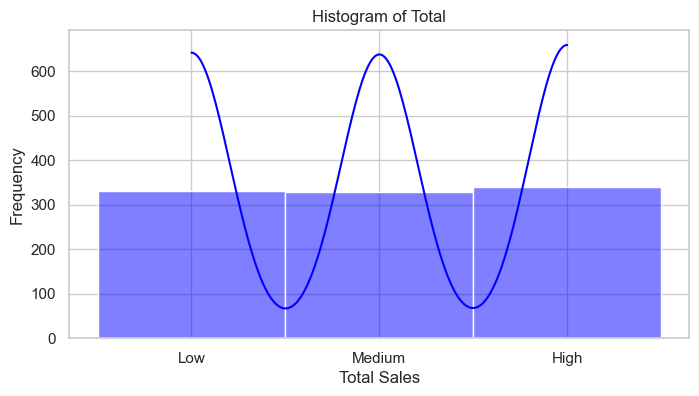
\includegraphics[width=0.5\textwidth]{Chapters/ch9/ch_9_w_graph.png}
    % \caption{Radar graph}
    % \label{fig:example}
\end{figure}
All 3 categories reach approximately equal highs and lows. This indicates that we have performed binning efficiently and can move onto the next step of the classification process.

\begin{figure}[h]
    \centering
    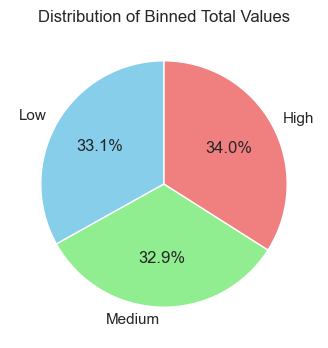
\includegraphics[width=0.3\textwidth]{Chapters/ch9/ch_9_piechart_1.png}
    % \caption{Radar graph}
    % \label{fig:example}
\end{figure}
This pie chart shows the spread of the categories High, Medium and Low as percentages of the ‘Total’ feature. It indicates that sampling is not required as these categories are roughly equal.

% ---------------------------------------------------------------------------------------------

\section{Splitting data }
Using Train-Test split, I split the dataset.  I already covered this step, in detail, during the preprocessing stage, so I won’t go into detail here.
\newline 
\newline 
Training set shape: (800, 22) (800,)
\newline 
Testing set shape: (200, 22) (200,)

% -----------------------------------------------------------------------------
\section{Model Training and Testing:}
Since the code after this is short, and applying the actual model is a small step, I decided to apply multiple models. Here are details about their obtained accuracy metrics:


\begin{table}[htbp]
    \centering
    \begin{adjustbox}{max width=\textwidth} % Fit the table to the page width
        \rowcolors{1}{green!20}{white} % Alternate row colors starting from the second row
        \rowcolors{2}{green!30}{white} % Slightly darker header row
        \begin{tabular}{|>{\columncolor{green!50}}c|c|c|c|c|}
            \hline
            \rowcolor{green!50} % Slightly darker header row color
            \textbf{Model} & \textbf{Accuracy} & \textbf{Precision} & \textbf{Recall} & \textbf{F1-Score} \\
            \hline
            \cellcolor{green!30}Random Forest  & 0.940 & 0.942260 &	0.940 &	0.940410\\
            \cellcolor{green!30}Gradient Boosting & 0.925 & 0.927232 &	0.925 & 0.925458 \\
            \cellcolor{green!30}Logistic Regression & 0.940	& 0.940435 & 0.940 & 0.939632 \\
            \cellcolor{green!30}Naive Bayes  & 0.920 & 0.921063 & 0.920 &	0.920297\\
            \cellcolor{green!30}K-Nearest Neighbors & 0.810	& 0.816504 &	0.810 &	0.812382 \\
            \cellcolor{green!30}Support Vector Machine & 0.915 & 0.914824 & 0.915 &	0.914877\\
            \hline
        \end{tabular}
    \end{adjustbox}
    % \caption{7 by 5 Table with alternating light green rows and a slightly darker green header}
    \label{tab:7x5_table}
\end{table}

\textbf{Key Findings:}
\begin{itemize}
\item Random Forest and Logistic Regression outperform other models with the highest accuracy of 94.0%.
\item Precision is consistently high across all models, indicating a low false positive rate in classifying customers.
\item Recall values are generally balanced, suggesting good performance in capturing true positive instances.
\item F1-Score combines precision and recall, showcasing the overall effectiveness of the model. Random Forest and Logistic Regression excel in this aspect.
\end{itemize}

\textbf{Conclusion}
Considering the high accuracy, precision, recall, and F1-Score, Random Forest or Logistic Regression is recommended for predicting customer segments based on purchasing behavior.





% Chapter 9

\chapter{Regression} % Main chapter title

\label{Chapter10} % For referencing the chapter elsewhere, use \ref{Chapter1} 

All previous preprocessing steps remain the same, the only difference is the exclusion of the process of binning since we need our target variable to be continuous for regression. I used the same target variable, ‘Total’. As I did with classification, I applied multiple models here too, since the process after preprocessing is quite short and straightforward. Applying multiple models helps gain useful insight into the problem, and it becomes easier to choose a good model for predictions.

\lhead{Chapter 10. \emph{Regression}} % This is for the header on each page - perhaps a shortened title

%----------------------------------------------------------------------------------------

\section{Evaluation Metrics:}

Unlike classification problems, where metrics like accuracy, precision, and recall are common, regression problems involve predicting continuous numerical values. Here, we justify the selection of Mean Squared Error (MSE), Root Mean Squared Error (RMSE), Mean Absolute Error (MAE), R-squared (R2), Adjusted R-squared (Adjusted R2), and Explained Variance as evaluation metrics.

\begin{itemize}
\item Mean Squared Error (MSE):
\newline 
MSE measures the average of the squared differences between predicted and actual values. It amplifies the impact of larger errors, providing a comprehensive view of overall model accuracy.
\item Root Mean Squared Error (RMSE):
\newline 
RMSE is the square root of MSE, providing an interpretable scale similar to the target variable. It helps in understanding the typical magnitude of errors in the predicted values.
\item Mean Absolute Error (MAE):
\newline 
MAE calculates the average absolute differences between predicted and actual values. It offers a more straightforward interpretation, treating all errors equally.
\item R-squared (R2):
\newline 
R2 quantifies the proportion of variance in the target variable explained by the model. A higher R2 indicates a better fit, with values closer to 1 indicating a stronger predictive capability.
\item Adjusted R-squared (Adjusted R2):
\newline 
Adjusted R2 adjusts for the number of predictors in the model, providing a more accurate reflection of model fit. It penalizes the addition of irrelevant predictors, addressing potential overfitting.
\item Explained Variance:
Explained Variance measures the proportion of variance in the target variable that the model accounts for. It complements R2, offering another perspective on the model's explanatory power.

\end{itemize}

\subsection{Why do we use different metrics for regression?}
\begin{itemize}

\item Continuous Prediction:
\newline
In regression, the goal is to predict numerical outcomes, making it inappropriate to use classification metrics designed for discrete class assignments.
\item
Quantitative Error Assessment:
\newline 
Regression metrics focus on quantifying the extent of errors between predicted and actual values, providing a nuanced understanding of model performance.

\end{itemize}


% ---------------------------------------------------------------------------------------

\section{Applying Regression:}
I made use of 5 different models, and 6 evaluation metrics, to help understand and evaluate the problem effectively. Here are the results:

\begin{table}[htbp]
    \centering
    \begin{adjustbox}{max width=\textwidth} % Fit the table to the page width
        \rowcolors{1}{green!20}{white} % Alternate row colors starting from the second row
        \rowcolors{2}{green!30}{white} % Slightly darker header row
        \begin{tabular}{|>{\columncolor{green!50}}c|c|c|c|c|c|c|}
            \hline
            \rowcolor{green!50} % Slightly darker header row color
            \textbf{Model} & \textbf{MSE} & \textbf{RMSE} & \textbf{MAE} & \textbf{R2} & \textbf{Adjusted R2} & \textbf{Explained Variance} \\
            \hline
            \cellcolor{green!30}Linear Regression & 405.263702 & 20.131162 & 14.938315 & 0.993771 & 0.993263 & 0.993788\\
            \cellcolor{green!30}Ridge &	405.359727 & 20.133547 & 14.947561 & 0.993769 &	0.993262 &	0.993787 \\
            \cellcolor{green!30}ElasticNet & 1366.993951 & 36.972881 & 27.411452 &	0.978989 &	0.977276 & 0.979146\\
            \cellcolor{green!30}Random Forest Regressor	& 302.036030 & 17.379184 & 13.506950 & 	0.995358 & 0.994979 & 0.995358\\
            \cellcolor{green!30}Decision Tree Regressor	& 637.420000 & 25.247178 & 19.150000 &	0.990203 & 0.989404 & 0.990238 \\
            \hline
        \end{tabular}
    \end{adjustbox}
    % \caption{7 by 5 Table with alternating light green rows and a slightly darker green header}
    \label{tab:7x5_table}
\end{table}

\section{Analysis}
\begin{itemize}
\item Linear Regression and Ridge Regression:
\newline
Both linear models (Linear Regression and Ridge Regression) exhibit excellent performance with low MSE, RMSE, and MAE, indicating a strong fit to the data.
The R² and Adjusted R² values are close to 1, suggesting that these models explain a high proportion of the variance in the target variable.
\item ElasticNet:
\newline
The ElasticNet model, while still performing reasonably well, shows higher errors compared to linear models. This could be due to the regularization applied, impacting the flexibility of the model.
\item Random Forest Regression:
\newline 
Random Forest Regression stands out as the top-performing model, with the lowest MSE, RMSE, and MAE. It demonstrates superior predictive accuracy and robustness, capturing complex relationships in the data.
\item Decision Tree Regression:
\newline
Decision Tree Regression performs well, but not as accurately as Random Forest. It exhibits slightly higher errors and lower R² values, indicating a lesser ability to explain the variance in the target variable.
\end{itemize}

\section{Conclusion}

Random Forest Regressor appears to be the most suitable for predicting sales and customer spending, providing a good balance between accuracy and generalization. The linear models (Linear Regression and Ridge Regression) also perform admirably. 











% Chapter 9

\chapter{Outlier Detection and Statistical Validation} % Main chapter title

\label{Chapter11} % For referencing the chapter elsewhere, use \ref{Chapter1} 

For this step, I'm going to be using encoded data, so that I'm able to apply the methods to all columns (since they are now numeric). Here is the DataFrame:

\begin{figure}[h]
    \centering
    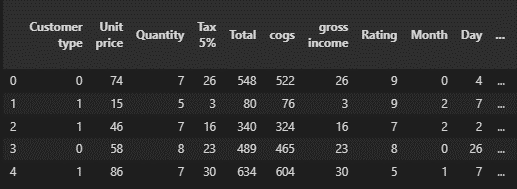
\includegraphics[width=1\textwidth]{Chapters/ch11/data_1.png}
    % \caption{This is an example image.}
    % \label{fig:example}
\end{figure}

\lhead{Chapter 11. \emph{Outlier Detection and Statistical Validation}} % This is for the header on each page - perhaps a shortened title

%----------------------------------------------------------------------------------------
Let’s consider the distinct value counts of all features, to get an idea of what we’re working with:

\begin{table}[htbp]
    \centering
    \begin{adjustbox}{max width=\textwidth} % Fit the table to the page width
        \rowcolors{1}{blue!20}{white} % Alternate row colors starting from the second row
        \rowcolors{2}{blue!30}{white} % Slightly darker header row
        \begin{tabular}{|>{\columncolor{blue!50}}c|c|}
            \hline
            \rowcolor{blue!50} % Slightly darker header row color
            \textbf{Customer type} & \textbf{Distinct Counts} \\
            \hline
            Unit price  & 90 \\
            Quantity  & 10 \\
            Tax 5\% & 49 \\
            Total & 546 \\
            COGS & 527 \\
            Gross income & 49 \\
            Rating & 7 \\
            Month & 3 \\
            Day & 31 \\
            Hour & 11 \\
            \verb|Branch_C| & 2 \\
            \verb|City_Naypyitaw| & 2\\
            \verb|City_Yangon| & 2 \\
            \verb|Gender_Male| & 2 \\
            \verb|Product line_Fashion accesories| & 2 \\
            \verb|Product line_Food and beverages| & 2 \\
            \verb|Product line_Health and beauty| & 2 \\
            \verb|Product line_Home and lifestyle| & 2 \\
            \verb|Product line_Sports and travel| & 2 \\
            \verb|Payment_Credit card| & 2 \\
            \verb|Payment_Ewallet| & 2 \\
            \hline
        \end{tabular}
    \end{adjustbox}
    % \caption{3 x 2 Table with alternating light green rows and a slightly darker green header}
    \label{tab:3x2_table}
\end{table}

All the encoded features have a distinct count of 2 since we used One-Hot encoding. Now, let’s move onto applying different methods for outlier detection.
% -----------------------------------------------------------------------------

\newpage
\section{Z-Score:}

\subsection{How does Z-Score work?}
\begin{equation}
Z = (X−mean)/std deviation
\end{equation}


The numerator $X - \mu$ calculates the difference between the individual data point ($X$) and the mean ($\mu$). This part of the formula measures how far the data point is from the center of the distribution. The result of the numerator is then divided by the standard deviation ($\sigma$). This division scales the difference in terms of standard deviations, providing a standardized measure of how far the data point is from the mean.

\newline 
A Z-score of 0 indicates that the data point's value is exactly at the mean. A positive Z-score indicates that the data point is above the mean, and the magnitude of the Z-score tells us how many standard deviations above the mean the data point is. A negative Z-score indicates that the data point is below the mean, and again, the magnitude represents how many standard deviations below the mean.

% -----------------------------------------------------------------------------------------------------------

\subsection{Applying Z-Score in code:}
In our code, we calculate the Z-score for each data point in selected columns of interest (e.g., Total, Unit price, Quantity) and identify outliers based on a user-defined threshold.

\lstset{language=Python}
\begin{lstlisting}
threshold_values = np.arange(1, 4, 0.5)
\end{lstlisting}

We must define a threshold value which will indicate the range for which we are considering the Z-score. The \verb|‘threshold_values’| is defined as an array ranging from 1 to 3. This array represents a range of threshold values that will be used in the outlier detection process.
\newline 
As well as this, we make use of ‘steps’ to identify outliers. The concept of using steps refers to the systematic exploration of different threshold values in the outlier detection process. Here, I made use of the Numpy function ‘arrange’ to define the number of steps, which I set at 0.5. Basically, the code will consider the dataset in increments of 0.5 (Threshold Value).
\newline 
The choice of starting from 1 and incrementing in steps of 0.5 allows for a nuanced exploration of outlier detection sensitivity. Lower thresholds may capture more points as outliers, while higher thresholds may only capture extreme anomalies.

% -------------------------------------------------------------------------------------------------------------------------------------------------------------------------------------------

\subsection{Result and Analysis:}

\definecolor{headercolor}{RGB}{255,128,0} % Define the header color (slightly darker orange)
\definecolor{rowcolor}{RGB}{255,218,185} % Define the row color (light orange)



\begin{table}[htbp]
\centering
\rowcolors{2}{rowcolor}{white} % Alternating row colors starting from the second row
\begin{adjustbox}{width=\textwidth}
\begin{tabular}{|c|c|c|c|c|c|c|c|c|}
\hline
\rowcolor{headercolor}
Threshold & Total & Customer type & Unit price & Quantity & Tax 5\% & Total & COGS & Gross Income \\
\hline
1.0 & 308 & 499 & 426 & 414 & 331 & 308 & 311 & 331 \\
1.5 & 112 & 0 & 139 & 231 & 112 & 112 & 112 & 112 \\
2.0 & 54 & 0 & 0 & 0 & 52 & 54 & 53 & 52 \\
2.5 & 17 & 0 & 0 & 0 & 11 & 17 & 17 & 11 \\
3.0 & 0 & 0 & 0 & 0 & 0 & 0 & 0 & 0 \\
3.5 & 0 & 0 & 0 & 0 & 0 & 0 & 0 & 0 \\
\hline
\end{tabular}
\end{adjustbox}
% \caption{A 7 by 9 table with alternating row colors}
\end{table}


As expected, increasing the threshold leads to a decrease in the number of identified outliers. At the highest threshold (3.5), no outliers are detected in any column, indicating a more conservative approach to outlier identification.

\begin{itemize}
\item Total: The 'Total' column consistently has a high number of outliers across different thresholds, suggesting potential anomalies in the overall sales amount.
\item Customer Type: The count of outliers for 'Customer type' is notably high at lower thresholds, indicating potential unusual patterns related to customer types.
\item Unit Price, Quantity, Tax 5\%: These columns show varying counts of outliers, suggesting potential discrepancies in pricing, purchase quantities, and tax amounts.
\item Rating: Outliers in the 'Rating' column decrease with higher thresholds, indicating that extreme ratings become less significant as the threshold increases.
\end{itemize}
\newline 
At certain thresholds, some columns have zero outliers. This is particularly evident for 'Hour' and 'Day,' which implies that these features might exhibit consistent patterns without significant outliers.


\begin{figure}[h]
    \centering
    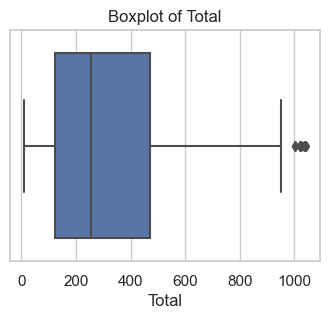
\includegraphics[width=0.5\textwidth]{Chapters/ch11/ch11_box_ploy_initial.png}
    % \caption{This is an example image.}
    % \label{fig:example}
\end{figure}

As can be observed, a certain number of outliers do seem to lie in the ‘Total’ column. 
\newline
I displayed all instances containing outliers in the column ‘Total’ and found these to be 17 rows in total.


\section{Interquartile Range:}
The Interquartile Range (IQR) is calculated as the difference between the third quartile (Q3) and the first quartile (Q1). This statistical measure is robust against extreme values and forms the basis for identifying outliers. The lower and upper bounds for potential outliers are established by extending 1.5 times the IQR below Q1 and above Q3, respectively. 
\newline
Upon applying this method, I obtained 9 outlier rows based on the ‘Total’ feature.

\begin{figure}[h]
    \centering
    \begin{subfigure}{0.5\textwidth}
        \centering
        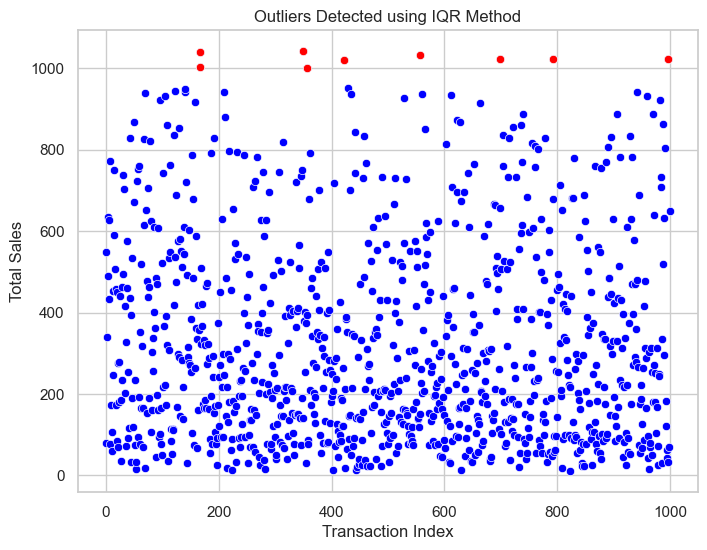
\includegraphics[width=\linewidth]{Chapters/ch11/ch_11_scatterplot.png}
        \caption{Scatterplot}
        \label{fig:scatterplot}
    \end{subfigure}%
    \begin{subfigure}{0.5\textwidth}
        \centering
        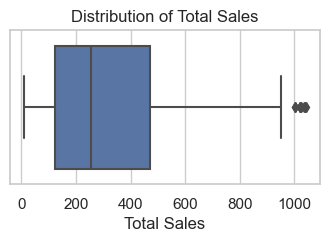
\includegraphics[width=\linewidth]{Chapters/ch11/ch_11_boxplot.png}
        \caption{Boxplot}
        \label{fig:boxplot}
    \end{subfigure}
    \caption{Two plots side by side}
    \label{fig:bothplots}
\end{figure}

% -----------------------------------------------------------------------------------------------
\newpage
\section{Isolation Forest:}
The Isolation Forest algorithm is a robust technique for identifying outliers or anomalies within a dataset, particularly adept at handling high-dimensional data efficiently. Its core concept revolves around the construction of isolation trees, binary trees that isolate data points by recursively partitioning the feature space. Anomalies, being rare instances, are expected to have shorter path lengths in these trees. The algorithm builds an ensemble of such trees and derives anomaly scores based on the average path length. Lower scores signify points that are easier to isolate and are thus more likely to be outliers.
\newline
The focus is on key dimensions such as 'Total', 'Unit price', 'Quantity', and 'cogs' columns, which are deemed crucial for understanding customer.
\newline 
\begin{lstlisting}[language=Python, frame=none]
model = IsolationForest(contamination=0.01)
\end{lstlisting}
\newline 
In the code above, a contamination parameter of 0.01 is set, indicating the proportion of outliers expected in the dataset. The Isolation Forest algorithm assigns an anomaly score to each data point, and those with a score indicative of an outlier (equal to -1) are isolated and extracted into a separate dataframe.
\newline 
A total of 10 rows are identified as outliers. Note that these are the top 1\% outliers in our dataset based on the following features: 'Total', 'Unit price', 'Quantity' and 'cogs'.
% -----------------------------------------------------------------------------------------------------------------------
\section{Statistical Validation:}
Statistical validation in the context of outlier detection involves applying formal statistical methods to assess and confirm the significance of identified outliers. It helps ensure that the patterns or anomalies observed in the data are not due to random chance and are, instead, statistically meaningful. The goal is to provide a robust foundation for drawing accurate conclusions from the detected outliers.

\subsection{ANOVA:}
Analysis of Variance is a statistical method used to compare means among multiple groups to determine if there are any statistically significant differences. It allows for the assessment of whether the variability within groups is comparable to the variability between groups. It is used to test the null hypothesis that there is no significant difference among the means of three or more groups. It also provides insights into whether any observed differences in means are likely due to genuine differences between groups or simply due to random variation.
\newline 
After making use of ANOVA in my code, I was unable to detect any significant patterns. Upon testing for both ‘Total’ and ‘Customer type’ features, I found no significant difference amongst the different categories of both features. This was indicated to me by the values of T-statistic and P-value, which ANOVA calculates. 

\subsection{Hypothesis Testing:}
In statistical validation, we often formulate hypotheses regarding the presence of outliers or patterns in the data.
\begin{itemize}
    \item Null Hypothesis (H0): Assumes that there are no significant outliers or patterns.
    \item Alternative Hypothesis (H1): Assumes the presence of significant outliers or patterns.
\end{itemize}
Hence in our case, the Null Hypothesis would be that there is no significant difference in total sales between normal transactions and outliers. And the Alternative Hypothesis would be that there is a significant difference in total sales between normal transactions and outliers.

\subsubsection{Two-Sample t-Test:}
\begin{itemize}
    \item T-Statistic: This measures the difference between the means of the two groups relative to the variability within each group. A higher absolute t-statistic suggests a greater difference between the groups.
    \item P-Value: The p-value represents the probability of obtaining the observed results (or more extreme) under the assumption that the null hypothesis is true. A lower p-value indicates stronger evidence against the null hypothesis.
\end{itemize}
So, in our case, the computed t-statistic is a quantitative measure of the difference in total sales between normal transactions and outliers. And our P-Value will indicate whether there is a significant difference in total sales. If there is, we will reject the null hypothesis.
\newline 
The significance level is denoted by alpha (α). This chosen level represents the threshold below which we would reject the null hypothesis. A common practice is to set alpha at 0.05, indicating a 5\% probability of rejecting the null hypothesis when it is true. Hence, I also set it at 0.05.

\begin{center}
\begin{tabular}{|c|c|}
\hline
\rowcolor{green!20} \textbf{T-Statistic} & \textbf{8.916895886005445} \\
\hline
\cellcolor{green!10} \textbf{P-Value} & \textbf{2.2421883966112505e-18} \\
\hline
\end{tabular}
\end{center}

With a p-value much smaller than the significance level, we reject the null hypothesis. Therefore, we conclude that there is a significant difference in total sales between normal transactions and outliers in our dataset.
\newline
The negative t-statistic indicates that outliers tend to have lower mean total sales compared to normal transactions. 






%-------------------------------------------------------------------------------
%	THESIS CONTENT - APPENDICES
%-------------------------------------------------------------------------------

\addtocontents{toc}{\vspace{2em}} % Add a gap in the Contents, for aesthetics

% \appendix % Cue to tell LaTeX that the following 'chapters' are Appendices

% Include the appendices of the thesis as separate files from the Appendices
% folder
% Uncomment the lines as you write the Appendices

% % Appendix A

\chapter{Appendix Title Here} % Main appendix title

\label{AppendixA} % For referencing this appendix elsewhere, use \ref{AppendixA}

\lhead{Appendix A. \emph{Appendix Title Here}} % This is for the header on each page - perhaps a shortened title

Write your Appendix content here.
%\input{Appendices/AppendixB}
%\input{Appendices/AppendixC}

\addtocontents{toc}{\vspace{2em}} % Add a gap in the Contents, for aesthetics

\backmatter

%-------------------------------------------------------------------------------
%	BIBLIOGRAPHY
%-------------------------------------------------------------------------------



% \documentclass{article}

% \addbibresource{Bibliography.bib} % references.bib is the file name

% \begin{document}


\chapter{References}
Here are some references to various documents and articles:

\begin{itemize}
  \item \href{https://pandas.pydata.org/pandas-docs/stable/}{Pandas Documentation} \cite{pandas}
  \item \href{https://scikit-learn.org/stable/}{Scikit-Learn Documentation} \cite{scikit-learn}
  \item \href{https://numpy.org/doc/stable/}{NumPy Documentation} \cite{numpy}
  \item \href{https://matplotlib.org/stable/contents.html}{Matplotlib Documentation} \cite{matplotlib}
  \item \href{https://seaborn.pydata.org/}{Seaborn Documentation} \cite{seaborn}
  \item \href{https://openai.com/chatgpt}{OpenAI ChatGPT} \cite{chatgpt}
  \item \href{https://bard.google.com/}{Google Bard} \cite{google_bard}
  \item \href{https://www.geeksforgeeks.org/interquartile-range-to-detect-outliers-in-data/}{Outliers Detection with IQR} \cite{iqr_outliers}
  \item \href{https://docs.scipy.org/doc/scipy/reference/generated/scipy.cluster.hierarchy.linkage.html}{Scipy Hierarchical Clustering} \cite{scipy_hierarchical_clustering}
  \item \href{https://towardsdatascience.com/understanding-boxplots-5e2df7bcbd51}{Understanding Boxplots} \cite{boxplots}
  \item \href{https://pymining.readthedocs.io/en/latest/index.html}{Pymining Documentation} \cite{pymining}
  \item \href{https://en.wikipedia.org/wiki/Sequential_Pattern_Mining}{Generalized Sequential Pattern (GSP) Algorithm} \cite{gsp_algorithm}
  \item \href{https://dl.acm.org/doi/10.1145/223784.223791}{Mining Sequential Patterns} \cite{agrawal1995mining}
  \item \href{https://www.geeksforgeeks.org/sequential-pattern-mining/}{Sequential Pattern Mining} \cite{sequential_pattern_mining}
  \item \href{https://en.wikipedia.org/wiki/Hierarchical_clustering#Agglomerative_hierarchical_clustering}{Agglomerative hierarchical clustering} \cite{agglomerative_clustering}
  \item \href{https://en.wikipedia.org/wiki/K-means_clustering}{K-means clustering} \cite{k_means}
  \item \href{https://en.wikipedia.org/wiki/K-medians_clustering}{K-medians clustering} \cite{k_medians}
  \item \href{https://en.wikipedia.org/wiki/Interquartile_range}{Interquartile Range (IQR) Method} \cite{iqr_method}
  \item \href{https://cs.nju.edu.cn/zhouzh/zhouzh.files/publication/icdm08b.pdf}{Isolation Forest} \cite{liu2008isolation}
  \item \href{https://en.wikipedia.org/wiki/DBSCAN}{DBSCAN} \cite{dbscan}
  \item \href{https://en.wikipedia.org/wiki/Mean_shift}{Mean shift} \cite{mean_shift}
  \item \href{https://www.borgelt.net/prefixspan/prefixspan.pdf}{PrefixSpan Documentation} \cite{prefixspan}
  \item \href{https://en.wikipedia.org/wiki/Principal_component_analysis}{Principal Component Analysis (PCA)} \cite{pca}
  \item \href{https://scikit-learn.org/stable/modules/generated/sklearn.decomposition.PCA.html}{Principal Component Analysis (PCA) - sklearn Documentation} \cite{pca_sklearn}
  \item \href{https://en.wikipedia.org/wiki/Apriori_algorithm}{Apriori Algorithm} \cite{apriori}
  \item \href{https://en.wikipedia.org/wiki/FP-growth}{FP-Growth Algorithm} \cite{fp_growth}
\end{itemize}

\printbibliography


\end{document}


\end{document}

